\documentclass[oneside, spanish]{book}
\usepackage[utf8]{inputenc}
\usepackage{geometry}
\geometry{verbose,a4paper,tmargin=2.5cm,bmargin=2.5cm,lmargin=2.5cm,rmargin=2.5cm}
\usepackage{fancyhdr}
\pagestyle{fancy}
\setcounter{tocdepth}{3}
\setlength{\parskip}{\medskipamount}
\setlength{\parindent}{0pt}
\usepackage{float}
\usepackage{framed}
\usepackage{amsthm}
\usepackage{amsmath}
\usepackage{graphicx}
\usepackage{wrapfig}
\usepackage{longtable}
\usepackage{color}
\usepackage[bookmarks]{hyperref}
\usepackage{listings}

\pretolerance=2000
\tolerance=3000
%%%%%%%%%%%%%%%%%%%%%%%%%%%%%% Textclass specific LaTeX commands.
\theoremstyle{plain}

%%%%%%%%%%%%%%%%%%%%%%%%%%%%%% User specified LaTeX commands.
\usepackage{fancyhdr}
    \pagestyle{fancy}
    \fancyhf{}
    \fancyhead[LO]{\leftmark} % En las páginas impares, parte izquierda del encabezado, aparecer el nombre de capítulo
    \fancyhead[RE]{\rightmark} % En las páginas pares, parte derecha del encabezado, aparecer el nombre de sección
    \fancyhead[RO,LE]{\thepage} % Nmeros de página en las esquinas de los encabezados
    \fancyfoot[RO]{José Luis Molina Soria}
    \fancyfoot[LO]{Editor de mapas mentales online con HTML5 y Javascript}
    \renewcommand{\chaptermark}[1]{\markboth{\textbf{\thechapter. #1}}{}} % Formato para el capítulo: N. Nombre
    \renewcommand{\sectionmark}[1]{\markright{\textbf{\thesection. #1}}} % Formato para la sección: N.M. Nombre
    \renewcommand{\headrulewidth}{0.6pt} % Ancho de la lnea horizontal bajo el encabezado
    \renewcommand{\footrulewidth}{0.6pt} % Ancho de la lnea horizontal sobre el pie (que en este ejemplo est vaco)
    \setlength{\headheight}{1.5\headheight} % Aumenta la altura del encabezado en una vez y media

\usepackage{babel}
\addto\shorthandsspanish{\spanishdeactivate{~<>}}

\renewcommand{\chaptername}{Parte} 
\renewcommand{\partname}{}
\renewcommand{\bibname}{BIBLIOGRAFÍA}


\makeatletter

\def\thickhrulefill{\leavevmode \leaders \hrule height 1ex \hfill \kern \z@}
\def\@makechapterhead#1{%
  \reset@font
  \parindent \z@ 
  \vspace*{10\p@}%
  \hbox{%
    \vbox{\hsize=2cm
      \begin{tabular}{c}
        \scshape \strut \@chapapp{} \\
        \fbox{%
          \vrule depth 10em width 0pt%
          \vrule height 0pt depth 0pt width 1ex%
          {\LARGE \bfseries \strut \thechapter}%
          \vrule height 0pt depth 0pt width 1ex%
          }
      \end{tabular}%
      }%
    \vbox{%
      \advance\hsize by -2cm
      \hrule\par
      \vskip 6pt%
      \hspace{0em}%
      \Huge \bfseries #1
      }%
    }%
  \vskip 100\p@
}
\def\@makeschapterhead#1{%
  \reset@font
  \parindent \z@ 
  \vspace*{10\p@}%
 \hbox{%
    \vbox{\hsize=2cm
      \begin{tabular}{c}
        \scshape \strut \vphantom{\@chapapp{}} \hphantom{\@chapapp{}} \\
        \fbox{%
          \vrule depth 10em width 0pt%
          \vrule height 0pt depth 0pt width 1ex%
          {\LARGE \bfseries \strut \hphantom{\thechapter}}%
          \vrule height 0pt depth 0pt width 1ex%
          }
      \end{tabular}%
      }%
    \vbox{%
      \advance\hsize by -2cm    
      \hrule\par
      \vskip 6pt%
      \hspace{1em}%
      \Huge \bfseries #1
      }%
    }%
  \vskip 100\p@
}


\usepackage{tocloft}
\renewcommand{\cftsecnumwidth}{3em}
%\renewcommand{\cftsecfont}{3em}
\renewcommand{\cftfignumwidth}{3em}
\setlength{\cftbeforesecskip}{0.7em \@plus\p@}
\setlength{\cftbeforefigskip}{0.4em \@plus\p@}
\renewcommand{\baselinestretch}{1.5}

\definecolor{lightgray}{rgb}{.9,.9,.9}
\definecolor{darkgray}{rgb}{.4,.4,.4}
\definecolor{purple}{rgb}{0.65, 0.12, 0.82}

\lstdefinelanguage{JavaScript}{
  keywords={typeof, new, true, false, catch, function, return, null, catch, switch, var, if, in, while, do, else, case, break},
  keywordstyle=\color{blue}\bfseries,
  ndkeywords={class, export, boolean, throw, implements, import, this},
  ndkeywordstyle=\color{darkgray}\bfseries,
  identifierstyle=\color{black},
  sensitive=false,
  comment=[l]{//},
  morecomment=[s]{/*}{*/},
  commentstyle=\color{purple}\ttfamily,
  stringstyle=\color{red}\ttfamily,
  morestring=[b]',
  morestring=[b]"
}

\lstset{
   language=JavaScript,
   backgroundcolor=\color{lightgray},
   extendedchars=true,
   inputencoding=ansinew,
   basicstyle=\linespread{0.90}\footnotesize\ttfamily,
   showstringspaces=false,
   showspaces=false,
   numbers=left,
   numberstyle=\footnotesize,
   numbersep=9pt,
   tabsize=2,
   breaklines=true,
   showtabs=false,
   captionpos=b
}

\begin{document} 
\lstset{inputencoding=utf8/latin1}

\setlength{\unitlength}{1 cm} 
\thispagestyle{empty}
\begin{center}
\textbf{\newline \newline \newline \large{UNIVERSIDAD DE MÁLAGA}}
\end{center}

\begin{center}
\textbf{\newline \large{ESCUELA TÉCNICA SUPERIOR DE INGENIERÍA INFORMÁTICA}}
\end{center}

\begin{center}
\textbf{\newline \large{INGENIERÍA TÉCNICA EN INFORMÁTICA DE GESTIÓN}}
\end{center}

\begin{center}
\textbf{\newline \newline \large{Editor de mapas mentales online con HTML5 y Javascript}}
\end{center}

\begin{center}
\textbf{\newline \newline Realizado por}

\textbf{José Luis Molina Soria}
\end{center}

\begin{center}
\textbf{\newline \newline Dirigido por}

\textbf{Juan Antonio Falgueras Cano}
\end{center}

\begin{center}
\textbf{\newline \newline Departamento}

\textbf{Lenguajes y Ciencias de la Computación}
\end{center}


\begin{flushright}
\textbf{\newline \newline \newline Málaga, \today}
\end{flushright}

\clearpage      











\newpage\mbox{}\thispagestyle{empty}

\begin{center}
\textbf{\newline \large{UNIVERSIDAD DE MÁLAGA}}

\textbf{\large{ESCUELA TÉCNICA SUPERIOR DE INGENIERÍA INFORMÁTICA}}
\newline \large{INGENIERÍA TÉCNICA EN INFORMÁTICA DE GESTIÓN}\newline
\end{center}


Reunido el tribunal examinador en el día de la fecha, constituido por: 

Presidente/a D$^{o}$/D$^{a}$. \underline{ }\underline{ }\underline{ }\underline{ }\underline{ }\underline{ }\underline{ }\underline{ }\underline{ }\underline{ }\underline{ }\underline{ }\underline{ }\underline{ }\underline{ }\underline{ }\underline{ }\underline{ }\underline{ }\underline{ }\underline{ }\underline{ }\underline{ }\underline{ }\underline{ }\underline{ }\underline{ }\underline{ }\underline{ }\underline{ }\underline{ }\underline{ }\underline{ }\underline{ }\underline{ }\underline{ }\underline{ }\underline{ }\underline{ }\underline{ }\underline{ }\underline{ }\underline{ }\underline{ }\underline{ }\underline{ }\underline{ }\underline{ }\underline{ }\underline{ }\underline{ }\underline{ }\underline{ }\underline{ }\underline{ }\underline{ }\underline{ }\underline{ }\underline{ }\underline{ }\underline{ }\underline{ }\underline{ }\underline{ }\underline{ }\underline{ }\underline{ }\underline{ }\underline{ }\underline{ }\underline{ }\underline{ }\underline{ }\underline{ }\underline{ }\underline{ }\underline{ }\underline{ }\underline{ }\underline{ }\underline{ }\underline{ }\underline{ }\underline{ }\underline{ }\underline{ }\underline{ }\underline{ }\underline{ }\underline{ }\underline{ }\underline{ }\underline{ }\underline{ }\underline{ }\underline{ }\underline{ }\underline{ }\underline{ }\underline{ }\underline{ }\underline{ }\underline{ }\underline{ }\underline{ }\underline{ }

Secretario/a D$^{o}$/D$^{a}$. \underline{ }\underline{ }\underline{ }\underline{ }\underline{ }\underline{ }\underline{ }\underline{ }\underline{ }\underline{ }\underline{ }\underline{ }\underline{ }\underline{ }\underline{ }\underline{ }\underline{ }\underline{ }\underline{ }\underline{ }\underline{ }\underline{ }\underline{ }\underline{ }\underline{ }\underline{ }\underline{ }\underline{ }\underline{ }\underline{ }\underline{ }\underline{ }\underline{ }\underline{ }\underline{ }\underline{ }\underline{ }\underline{ }\underline{ }\underline{ }\underline{ }\underline{ }\underline{ }\underline{ }\underline{ }\underline{ }\underline{ }\underline{ }\underline{ }\underline{ }\underline{ }\underline{ }\underline{ }\underline{ }\underline{ }\underline{ }\underline{ }\underline{ }\underline{ }\underline{ }\underline{ }\underline{ }\underline{ }\underline{ }\underline{ }\underline{ }\underline{ }\underline{ }\underline{ }\underline{ }\underline{ }\underline{ }\underline{ }\underline{ }\underline{ }\underline{ }\underline{ }\underline{ }\underline{ }\underline{ }\underline{ }\underline{ }\underline{ }\underline{ }\underline{ }\underline{ }\underline{ }\underline{ }\underline{ }\underline{ }\underline{ }\underline{ }\underline{ }\underline{ }\underline{ }\underline{ }\underline{ }\underline{ }\underline{ }\underline{ }\underline{ }\underline{ }\underline{ }\underline{ }\underline{ }\underline{ }\underline{ }

Vocal D$^{o}$/D$^{a}$. \underline{ }\underline{ }\underline{ }\underline{ }\underline{ }\underline{ }\underline{ }\underline{ }\underline{ }\underline{ }\underline{ }\underline{ }\underline{ }\underline{ }\underline{ }\underline{ }\underline{ }\underline{ }\underline{ }\underline{ }\underline{ }\underline{ }\underline{ }\underline{ }\underline{ }\underline{ }\underline{ }\underline{ }\underline{ }\underline{ }\underline{ }\underline{ }\underline{ }\underline{ }\underline{ }\underline{ }\underline{ }\underline{ }\underline{ }\underline{ }\underline{ }\underline{ }\underline{ }\underline{ }\underline{ }\underline{ }\underline{ }\underline{ }\underline{ }\underline{ }\underline{ }\underline{ }\underline{ }\underline{ }\underline{ }\underline{ }\underline{ }\underline{ }\underline{ }\underline{ }\underline{ }\underline{ }\underline{ }\underline{ }\underline{ }\underline{ }\underline{ }\underline{ }\underline{ }\underline{ }\underline{ }\underline{ }\underline{ }\underline{ }\underline{ }\underline{ }\underline{ }\underline{ }\underline{ }\underline{ }\underline{ }\underline{ }\underline{ }\underline{ }\underline{ }\underline{ }\underline{ }\underline{ }\underline{ }\underline{ }\underline{ }\underline{ }\underline{ }\underline{ }\underline{ }\underline{ }\underline{ }\underline{ }\underline{ }\underline{ }\underline{ }\underline{ }\underline{ }\underline{ }\underline{ }\underline{ }\underline{ }\underline{ }\underline{ }\underline{ }\underline{ }\underline{ }\underline{ }\underline{ }\underline{ }\underline{ }

para juzgar el proyecto Fin de Carrera titulado: \underline{ }\underline{ }\underline{ }\underline{ }\underline{ }\underline{ }\underline{ }\underline{ }\underline{ }\underline{ }\underline{ }\underline{ }\underline{ }\underline{ }\underline{ }\underline{ }\underline{ }\underline{ }\underline{ }\underline{ }\underline{ }\underline{ }\underline{ }\underline{ }\underline{ }\underline{ }\underline{ }\underline{ }\underline{ }\underline{ }\underline{ }\underline{ }\underline{ }\underline{ }\underline{ }\underline{ }\underline{ }\underline{ }\underline{ }\underline{ }\underline{ }\underline{ }\underline{ }\underline{ }\underline{ }\underline{ }\underline{ }\underline{ }\underline{ }\underline{ }\underline{ }\underline{ }\underline{ }\underline{ }\underline{ }\underline{ }\underline{ }\underline{ }\underline{ }\underline{ }\underline{ }\underline{ }\underline{ }\underline{ }\underline{ }\underline{ }\underline{ }\underline{ }\underline{ }\underline{ }\underline{ }

\underline{ }\underline{ }\underline{ }\underline{ }\underline{ }\underline{ }\underline{ }\underline{ }\underline{ }\underline{ }\underline{ }\underline{ }\underline{ }\underline{ }\underline{ }\underline{ }\underline{ }\underline{ }\underline{ }\underline{ }\underline{ }\underline{ }\underline{ }\underline{ }\underline{ }\underline{ }\underline{ }\underline{ }\underline{ }\underline{ }\underline{ }\underline{ }\underline{ }\underline{ }\underline{ }\underline{ }\underline{ }\underline{ }\underline{ }\underline{ }\underline{ }\underline{ }\underline{ }\underline{ }\underline{ }\underline{ }\underline{ }\underline{ }\underline{ }\underline{ }\underline{ }\underline{ }\underline{ }\underline{ }\underline{ }\underline{ }\underline{ }\underline{ }\underline{ }\underline{ }\underline{ }\underline{ }\underline{ }\underline{ }\underline{ }\underline{ }\underline{ }\underline{ }\underline{ }\underline{ }\underline{ }\underline{ }\underline{ }\underline{ }\underline{ }\underline{ }\underline{ }\underline{ }\underline{ }\underline{ }\underline{ }\underline{ }\underline{ }\underline{ }\underline{ }\underline{ }\underline{ }\underline{ }\underline{ }\underline{ }\underline{ }\underline{ }\underline{ }\underline{ }\underline{ }\underline{ }\underline{ }\underline{ }\underline{ }\underline{ }\underline{ }\underline{ }\underline{ }\underline{ }\underline{ }\underline{ }\underline{ }\underline{ }\underline{ }\underline{ }\underline{ }\underline{ }\underline{ }\underline{ }\underline{ }\underline{ }\underline{ }\underline{ }\underline{ }\underline{ }\underline{ }\underline{ }\underline{ }\underline{ }\underline{ }\underline{ }\underline{ }\underline{ }\underline{ }\underline{ }\underline{ }\underline{ }\underline{ }\underline{ }\underline{ }

\underline{ }\underline{ }\underline{ }\underline{ }\underline{ }\underline{ }\underline{ }\underline{ }\underline{ }\underline{ }\underline{ }\underline{ }\underline{ }\underline{ }\underline{ }\underline{ }\underline{ }\underline{ }\underline{ }\underline{ }\underline{ }\underline{ }\underline{ }\underline{ }\underline{ }\underline{ }\underline{ }\underline{ }\underline{ }\underline{ }\underline{ }\underline{ }\underline{ }\underline{ }\underline{ }\underline{ }\underline{ }\underline{ }\underline{ }\underline{ }\underline{ }\underline{ }\underline{ }\underline{ }\underline{ }\underline{ }\underline{ }\underline{ }\underline{ }\underline{ }\underline{ }\underline{ }\underline{ }\underline{ }\underline{ }\underline{ }\underline{ }\underline{ }\underline{ }\underline{ }\underline{ }\underline{ }\underline{ }\underline{ }\underline{ }\underline{ }\underline{ }\underline{ }\underline{ }\underline{ }\underline{ }\underline{ }\underline{ }\underline{ }\underline{ }\underline{ }\underline{ }\underline{ }\underline{ }\underline{ }\underline{ }\underline{ }\underline{ }\underline{ }\underline{ }\underline{ }\underline{ }\underline{ }\underline{ }\underline{ }\underline{ }\underline{ }\underline{ }\underline{ }\underline{ }\underline{ }\underline{ }\underline{ }\underline{ }\underline{ }\underline{ }\underline{ }\underline{ }\underline{ }\underline{ }\underline{ }\underline{ }\underline{ }\underline{ }\underline{ }\underline{ }\underline{ }\underline{ }\underline{ }\underline{ }\underline{ }\underline{ }\underline{ }\underline{ }\underline{ }\underline{ }\underline{ }\underline{ }\underline{ }\underline{ }\underline{ }\underline{ }\underline{ }\underline{ }\underline{ }\underline{ }\underline{ }\underline{ }\underline{ }\underline{ }


del alumno/a D$^{o}$/D$^{a}$ : \underline{ }\underline{ }\underline{ }\underline{ }\underline{ }\underline{ }\underline{ }\underline{ }\underline{ }\underline{ }\underline{ }\underline{ }\underline{ }\underline{ }\underline{ }\underline{ }\underline{ }\underline{ }\underline{ }\underline{ }\underline{ }\underline{ }\underline{ }\underline{ }\underline{ }\underline{ }\underline{ }\underline{ }\underline{ }\underline{ }\underline{ }\underline{ }\underline{ }\underline{ }\underline{ }\underline{ }\underline{ }\underline{ }\underline{ }\underline{ }\underline{ }\underline{ }\underline{ }\underline{ }\underline{ }\underline{ }\underline{ }\underline{ }\underline{ }\underline{ }\underline{ }\underline{ }\underline{ }\underline{ }\underline{ }\underline{ }\underline{ }\underline{ }\underline{ }\underline{ }\underline{ }\underline{ }\underline{ }\underline{ }\underline{ }\underline{ }\underline{ }\underline{ }\underline{ }\underline{ }\underline{ }\underline{ }\underline{ }\underline{ }\underline{ }\underline{ }\underline{ }\underline{ }\underline{ }\underline{ }\underline{ }\underline{ }\underline{ }\underline{ }\underline{ }\underline{ }\underline{ }\underline{ }\underline{ }\underline{ }\underline{ }\underline{ }\underline{ }\underline{ }\underline{ }\underline{ }\underline{ }\underline{ }\underline{ }\underline{ }\underline{ }\underline{ }\underline{ }\underline{ }\underline{ }

dirigido por D$^{o}$/D$^{a}$ : \underline{ }\underline{ }\underline{ }\underline{ }\underline{ }\underline{ }\underline{ }\underline{ }\underline{ }\underline{ }\underline{ }\underline{ }\underline{ }\underline{ }\underline{ }\underline{ }\underline{ }\underline{ }\underline{ }\underline{ }\underline{ }\underline{ }\underline{ }\underline{ }\underline{ }\underline{ }\underline{ }\underline{ }\underline{ }\underline{ }\underline{ }\underline{ }\underline{ }\underline{ }\underline{ }\underline{ }\underline{ }\underline{ }\underline{ }\underline{ }\underline{ }\underline{ }\underline{ }\underline{ }\underline{ }\underline{ }\underline{ }\underline{ }\underline{ }\underline{ }\underline{ }\underline{ }\underline{ }\underline{ }\underline{ }\underline{ }\underline{ }\underline{ }\underline{ }\underline{ }\underline{ }\underline{ }\underline{ }\underline{ }\underline{ }\underline{ }\underline{ }\underline{ }\underline{ }\underline{ }\underline{ }\underline{ }\underline{ }\underline{ }\underline{ }\underline{ }\underline{ }\underline{ }\underline{ }\underline{ }\underline{ }\underline{ }\underline{ }\underline{ }\underline{ }\underline{ }\underline{ }\underline{ }\underline{ }\underline{ }\underline{ }\underline{ }\underline{ }\underline{ }\underline{ }\underline{ }\underline{ }\underline{ }\underline{ }\underline{ }\underline{ }\underline{ } , 

y, en su caso, dirigido académicamente por D$^{o}$/D$^{a}$ : \underline{ }\underline{ }\underline{ }\underline{ }\underline{ }\underline{ }\underline{ }\underline{ }\underline{ }\underline{ }\underline{ }\underline{ }\underline{ }\underline{ }\underline{ }\underline{ }\underline{ }\underline{ }\underline{ }\underline{ }\underline{ }\underline{ }\underline{ }\underline{ }\underline{ }\underline{ }\underline{ }\underline{ }\underline{ }\underline{ }\underline{ }\underline{ }\underline{ }\underline{ }\underline{ }\underline{ }\underline{ }\underline{ }\underline{ }\underline{ }\underline{ }\underline{ }\underline{ }\underline{ }\underline{ }\underline{ }\underline{ }\underline{ }\underline{ }\underline{ }\underline{ }\underline{ }\underline{ }\underline{ }\underline{ }\underline{ }\underline{ }\underline{ }\underline{ }\underline{ }\underline{ }\underline{ }\underline{ }\underline{ }\underline{ }\underline{ }

\underline{ }\underline{ }\underline{ }\underline{ }\underline{ }\underline{ }\underline{ }\underline{ }\underline{ }\underline{ }\underline{ }\underline{ }\underline{ }\underline{ }\underline{ }\underline{ }\underline{ }\underline{ }\underline{ }\underline{ }\underline{ }\underline{ }\underline{ }\underline{ }\underline{ }\underline{ }\underline{ }\underline{ }\underline{ }\underline{ }\underline{ }\underline{ }\underline{ }\underline{ }\underline{ }\underline{ }\underline{ }\underline{ }\underline{ }\underline{ }\underline{ }\underline{ }\underline{ }\underline{ }\underline{ }\underline{ }\underline{ }\underline{ }\underline{ }\underline{ }\underline{ }\underline{ }\underline{ }\underline{ }\underline{ }\underline{ }\underline{ }\underline{ }\underline{ }\underline{ }\underline{ }\underline{ }\underline{ }\underline{ }\underline{ }\underline{ }\underline{ }\underline{ }\underline{ }\underline{ }\underline{ }\underline{ }\underline{ }\underline{ }\underline{ }\underline{ }\underline{ }\underline{ }\underline{ }\underline{ }\underline{ }\underline{ }\underline{ }\underline{ }\underline{ }\underline{ }\underline{ }\underline{ }\underline{ }\underline{ }\underline{ }\underline{ }\underline{ }\underline{ }\underline{ }\underline{ }\underline{ }\underline{ }\underline{ }\underline{ }\underline{ }\underline{ }\underline{ }\underline{ }\underline{ }\underline{ }\underline{ }\underline{ }\underline{ }\underline{ }\underline{ }\underline{ }\underline{ }\underline{ }\underline{ }\underline{ }\underline{ }\underline{ }\underline{ }\underline{ }\underline{ }\underline{ }\underline{ }\underline{ }\underline{ }\underline{ }\underline{ }\underline{ }\underline{ }\underline{ }\underline{ }\underline{ }\underline{ }\underline{ }\underline{ }

ACORDÓ POR \underline{ }\underline{ }\underline{ }\underline{ }\underline{ }\underline{ }\underline{ }\underline{ }\underline{ }\underline{ }\underline{ }\underline{ }\underline{ }\underline{ }\underline{ }\underline{ }\underline{ }\underline{ }\underline{ }\underline{ }\underline{ }\underline{ }\underline{ }\underline{ }\underline{ }\underline{ }\underline{ }\underline{ }\underline{ }\underline{ }\underline{ }\underline{ }\underline{ }\underline{ }\underline{ }\underline{ }\underline{ }\underline{ }\underline{ }\underline{ }\underline{ }\underline{ }\underline{ }\underline{ }\underline{ }\underline{ }\underline{ }\underline{ }\underline{ }\underline{ }\underline{ }\underline{ }\underline{ }\underline{ }\underline{ }\underline{ }\underline{ }\underline{ }\underline{ }\underline{ }\underline{ }\underline{ }\underline{ }\underline{ }\underline{ }\underline{ }\underline{ }\underline{ }\underline{ } OTORGAR LA CALIFICACIÓN 

DE \underline{ }\underline{ }\underline{ }\underline{ }\underline{ }\underline{ }\underline{ }\underline{ }\underline{ }\underline{ }\underline{ }\underline{ }\underline{ }\underline{ }\underline{ }\underline{ }\underline{ }\underline{ }\underline{ }\underline{ }\underline{ }\underline{ }\underline{ }\underline{ }\underline{ }\underline{ }\underline{ }\underline{ }\underline{ }\underline{ }\underline{ }\underline{ }\underline{ }\underline{ }\underline{ }\underline{ }\underline{ }\underline{ }\underline{ }\underline{ }\underline{ }\underline{ }\underline{ }\underline{ }\underline{ }\underline{ }\underline{ }\underline{ }\underline{ }\underline{ }\underline{ }\underline{ }\underline{ }\underline{ }\underline{ }\underline{ }

\vspace{10mm}

Y PARA QUE CONSTE, SE EXTIENDE FIRMADA POR LOS COMPARECIENTES DEL TRIBUNAL, LA PRESENTE DILIGENCIA 

\begin{flushright}Málaga a \underline{ }\underline{ }\underline{ }\underline{ } de \underline{ }\underline{ }\underline{ }\underline{ }\underline{ }\underline{ }\underline{ }\underline{ }\underline{ }\underline{ }\underline{ }\underline{ }\underline{ }\underline{ }\underline{ }\underline{ }\underline{ }\underline{ }\underline{ } de 20\underline{ }\underline{ }\underline{ }\underline{ }
\end{flushright}

\vspace{20mm}


\begin{center}
El/La Presidente/a \,\,\,\,\,\,\,\,\,\,\,\,\,\,\,\,\,\,\,\,\,\,\,\,\,\,\,\,\,\,\,\,\,\,\,\,\,\,\,\,\,\,\,\, El/La Secretario/a\,\,\,\,\,\,\,\,\,\,\,\,\,\,\,\,\,\,\,\,\,\,\,\,\,\,\,\,\,\,\,\,\,\,\,\,\,\,\,\,\,\,\,\,El/La Vocal
\end{center}

\vspace{20mm}

\begin{center}
Fdo: \,\,\,\,\,\,\,\,\,\,\,\,\,\,\,\,\,\,\,\,\,\,\,\,\,\,\,\,\,\,\,\,\,\,\,\,\,\,\,\,\,\,\,\,\,\,\,\,\,\,\,\,\,\,\,\,\,\,\,\,\,\,\,\,\,\,\,\,\,\,\,\,\,\,\,\,\,\,\,\,\,\,\,\, Fdo: \,\,\,\,\,\,\,\,\,\,\,\,\,\,\,\,\,\,\,\,\,\,\,\,\,\,\,\,\,\,\,\,\,\,\,\,\,\,\,\,\,\,\,\,\,\,\,\,\,\,\,\,\,\,\,\,\,\,\,\,\,\,\,\,\,\,\,\,\,\,\,\,\,\,\,\,\, Fdo: \,\,\,\,\,\,\,\,\,\,\,\,\,\,\,\,\,\,\,
\end{center}

\clearpage

\newpage
          


\newcommand{\cdpchapter}[1]{\cleardoublepage\chapter*{#1}}

\setcounter{page}{1}


\fontsize{12}{16}
\begin{flushright}

\vspace{80mm}

\textit{\textbf{Agradecimientos}}
\end{flushright}
\begin{flushright}
\textit{\textbf{A mi familia y padres por su paciencia}}
\end{flushright}
\newpage
\renewcommand{\contentsname}{Tabla de contenidos}
\setcounter{tocdepth}{1} 
\tableofcontents
\newpage
\setcounter{tocdepth}{2} 
\listoffigures
%\renewcommand{\contentsname}{\'Indice general}
%\setcounter{tocdepth}{2} 
%\tableofcontents 


\newpage\mbox{}\thispagestyle{empty}

\chapter{Abstract}

El editor de mapas mentales on-line es un sistema web desarrollado única y exclusivamente en HTML5
para diseñar y elaborar mapas mentales con formato FreeMind. Formato el cual, es considerado un
estándar en el mundo de los mapas mentales.

La idea que subyace en la realización de este editor de mapas mentales, es probar las nuevas
tecnologías existentes alrededor de HTML5 y comprobar el estado actual de dicha
tecnología tras el interés y la relevancia que está adquiriendo en estos últimos años. 

La metodología Ágil, utilizada para llevar a cabo el proyecto, se adapta muy bien al desarrollo web. Permitiendo un feedback constante desde la versión inicial hasta la actual. Conjuntamente con la metodología Ágil se utilizado otras metodologías y paradigmas de programación como el BBD\footnote{Como sistema de pruebas y verificación del código fuente}, patrones de diseño, etc ... También se ha hecho uso de tecnologías ya existentes como soporte al desarrollo, entre ellas destacar KineticJS, Mocha, GruntJS, NodeJS, JSHint, JSDoc y GitHub. Todas estas tecnologías han propiciado una experiencia de desarrollo satisfactoria. 

En resumen, se ha podido constatar un gran avance en HTML5 con respecto a la versión anterior. A pesar de ello, sigue existiendo, aunque en mucho menor grado, una gran dependencia con el navegador. 


\newpage\mbox{}\thispagestyle{empty}

\chapter{Motivación y objetivos}


\section{Motivación}

Desde hace ya unos años, estamos viviendo una revolución en el desarrollo web, que a provocado un cambio en nuestro estilo de vida, la forma de comunicarnos, en los flujos de información e incluso en nuestras relaciones diarias. HTML\footnote{Hypertext Markup Language} y JavaScript son una parte importante de esta revolución, y es por ello, que decidí dar el paso y crear una aplicación que funcionará única y exclusivamente en el navegador (sin necesidad de un servidor). 

Estamos viendo como día a día, aplicaciones que han sido por antonomasia nativas (editores de texto, hojas de cálculo, aplicaciones de gestión, juegos ...), están siendo implementadas con tecnologías web con gran éxito. Los editores de mapas mentales también han dado ese paso existen aplicaciones como text2mindmap\footnote{http://www.text2mindmap.com/}, MindMeister\footnote{http://www.mindmeister.com/es}, etc., tan versátiles o más que las propias aplicaciones nativas.

Hace ya tiempo que vio la luz los primeros borradores de HTML5\footnote{El primer borrador de HTML5 fue publicado en 2008} (ver figura \ref{fig:html5}) pero su implantación está siendo lenta, no sólo por parte de la comunidad de desarrolladores y diseñadores, sino también por parte de los navegadores. 

HTML5 ha tomado en cuenta los defectos de su versión anterior\footnote{HTML 4.01} y mejorar otras características como: 

\begin{figure}[htbp]
\centering
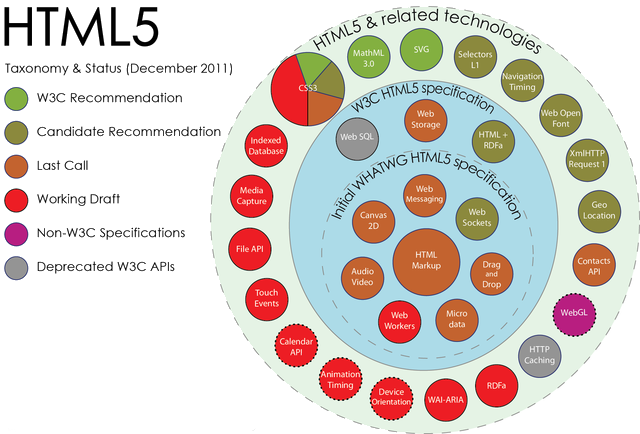
\includegraphics[width=1.1\textwidth]{imagenes/html5}
\caption{Esquema general de la especificación HTML5 a diciembre de 2011}
\label{fig:html5}
\end{figure}


\begin{itemize}
\item \textbf{Nuevas etiquetas estructurales.} Se ha incorporado un nuevo conjunto de etiquetas pensadas para definir mejor la estructura de una web, entre las más importantes están las de encabezado, barra de navegación, secciones y pie.

\item \textbf{Manejo de imágenes.} En la versión anterior podía incorporar imágenes ahora, además podemos modificarlas e interactuar con ellas. También disponemos un una etiqueta y un API completo para manejo de canvas\footnote{En principio, sólo en 2D.}.

\item \textbf{Etiquetas de vídeo y audio.} Sin incluir flash ni aplicaciones externas podemos incorporar un reproductor de vídeo y/o audio. 

\item \textbf{Mejora en la semántica web.} HTML5 incluye elementos que permiten dar información de la página web a los buscadores para obtener resultados adaptados a las necesidades del usuario.

\item \textbf{Soporte móvil/tabletas.} Mejoras en las hojas de estilos, nuevos manejadores para evento touch, etc.

\item \textbf{Acceso a ficheros.} Incorpora un API para lectura/escritura de ficheros.
  
\end{itemize}

La motivación no puede ser otra que profundizar en las características de HTML5 y aprender de esta tecnología. 

\section{Objetivos}

El principal objetivo de este proyecto es la creación de un editor de mapas mentales online. El editor, frontend, debe ejecutarse completamente en el cliente. Para ello, vamos a utilizar como lienzo de dibujos el canvas de HTML5 y Javascript como lenguaje de desarrollo. 

El usuario podrá navegar por el diagrama con los cursores partiendo desde la idea central. Interactuará con el diagrama de forma que, dependiendo del nodo en el que se encuentre y la acción que realice podrá insertar, modificar, anotar, plegar, etc...

Esta fuerte interacción, provoca que dentro de los objetivos del proyecto, se encuentre la elaboración de una  extensa librería JavaScript, bien estructurada y testeada. 

En todo momento, y en pos de una aplicación lo más estándar posible, se seguirá las especificaciones de la World Wide Web Consortium\footnote{Web oficial de la W3C http://www.w3.org/} (W3C) y la especificación 

Como objetivo principal está pues, la universalidad, independencia de sistemas y la inmediatez de uso, sin instalación, siempre actualizada, e incluso la posibilidad de uso en forma local con cualquier navegador actual que sigue el estándar HTML5.  Entre las posibles plataformas de uso se tratará de incluir las plataformas táctiles, especialmente los tablets.

%\section{Organización de la memoria}
%
%El presente documento esta divido en los siguiente capítulos.
%
%\begin{enumerate}
%\item Introducción. \newline
%Descripción general del proyecto y exposición de la estructura de la memoria. 
%
%\item Mapas mentales. \newline
%Apartado para descubrir que es, historia y usos de los mapas mentales. 
%
%\item Diseño e implementación. \newline
%En este capítulo se muestra la metodología, diseño, estudio e implementaciones para llevar a cabo la realización del proyecto.  
%
%\item Herramientas utilizadas. \newline
%Descripción de todas y cada una de las herramientas utilizas en el desarrollo del proyecto.
%
%\item Manual de usuarios. \newline
%Manual para el usuario final. 
%
%\item Conclusiones. \newline
%Capítulo para la conclusiones finales e impresiones.
%
%\end{enumerate}


\newpage\mbox{}\thispagestyle{empty}

\chapter{Introducción}

En la introducción al tema se presentará precisa y concisamente la situación actual de 
   la disciplina tratado por el TFM (aquí sí que suele haber gran número de referencias 
   bibliográficas relevantes que introduzcan y lleven a los últimos avances o estado o 
   situación actual del tema).
   La descripción de la situación actual del tema debe ser breve y con referencias.
   Destacar, si es el caso, cualquier información relativa a los aspectos interdisciplinares o 
   multidisciplinares que surjan y se contemplen en el trabajo aunque no se desarrollen, 
   pero sí se referencian.

   Dentro de la introducción se debe terminar especificando hasta dónde llega la 
   investigación previa que haya guiado a la aportada.
   
   Aclarar su relación con líneas anteriores del estado de la cuestión.

\section{¿Qué es?}

Los mapa mentales son un método efectivamente sencillo de asimilar y memorizar información a través de la representación visual de la información. 

Por naturaleza, nuestro celebro tiene un potencial ilimitado y que, en muchas ocasiones es desaprovechado o difícil de interpretar. Tenemos dos hemisferios el izquierdo y el derecho, el racional y el creativo, ambos funcionan de forma separada. Los mapas mentales consiguen relacionar ambos hemisferios (racional y creativo) y lograr que funcionen conjuntamente. 

Toda persona tiene una forma natural de elaborar sus propias ideas, mediante pensamiento irradiante\footnote{que irradia} . El pensamiento irradiante refleja mediante la asociación de ideas nuestros pensamientos y conocimientos sobre una materia concreta.  A esta forma de pensamiento podemos acceder mediante los mapas mentales, que irradian y asocian ideas a partir de un concepto central. 

\begin{figure}[htbp]
\centering
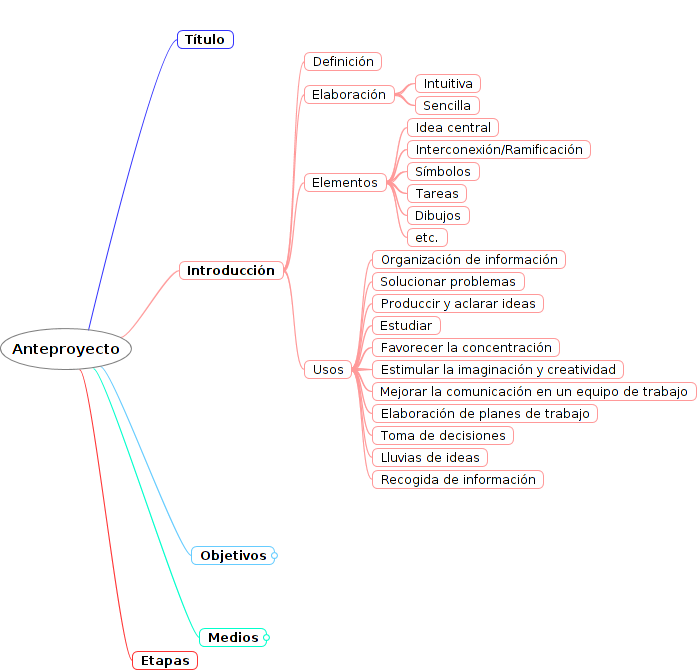
\includegraphics[width=0.9\textwidth]{imagenes/freemind}
\caption{Mapa mental de FreeMind}
\label{fig:freemind}
\end{figure}



\section{Aplicaciones y beneficios.}

Los campos de aplicación y los beneficios de los mapas mentales son muchos y muy diversos. Entre los más destacados tenemos:

\begin{itemize}
\item Estimular la memoria, imaginación y creatividad.
\item Organizar información.
\item Concentrarnos en la resolución de un problema.
\item Tomar notas y apuntes.
\item Producir y aclarar ideas o conceptos. 
\item Visualizar escenarios complejos.
\item Consolidar procesos de estudios y aprendizaje.
\item Favorecer la concentración.
\item Proyectos. Organizar el proyecto y priorizar el plan de trabajo.
\item Mejorar la comunicación en un equipo de trabajo.
\item Preparar y dirigir una reunión.
\item Toma de decisiones.
\item Lluvias de ideas.
\item Recogida de información.
\item Expresar ideas complejas y difíciles de redactar.
\item Diseñar el contenido de un escrito o informe.
\item Preparar una presentación en público.
\item Elaboración de sitios webs.
\end{itemize}


\section{Partes de un mapa mental.}

\subsection{Según su estructura.}
Un mapa mental tiene las siguientes estructuras esenciales (figura \ref{fig:partesestructura}):

\begin{enumerate}
\item Idea central.
\item Aristas. Establece una asociación de ideas.
\item Nodo. Ideas segundarías o asociada a otra idea.
\end{enumerate}

\begin{figure}[htbp]
\centering
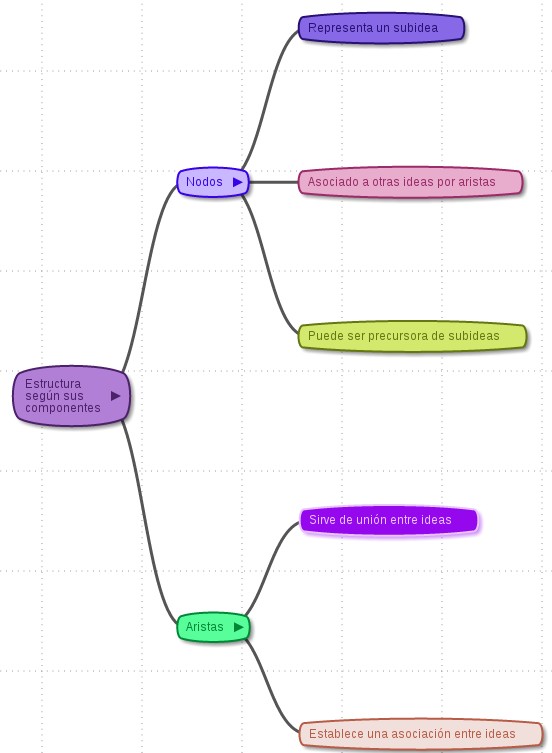
\includegraphics[width=0.6\textwidth]{imagenes/Estructura2.png}
\caption{Partes de un mapa mental}
\label{fig:partesestructura}
\end{figure}

\subsection{Por contenido.}

Un mapa mental podemos estructurarlo según su contenido (figura \ref{fig:partescontenido}).

\begin{enumerate}
\item Idea central
\item Los temas principales del asunto irradian de la imagen central como ramas.
\item Cada rama contiene una imagen o una palabra clave asociada.
\item Las ramas forman una estructura nodal conectada.
\end{enumerate}

\begin{figure}[htbp]
\centering
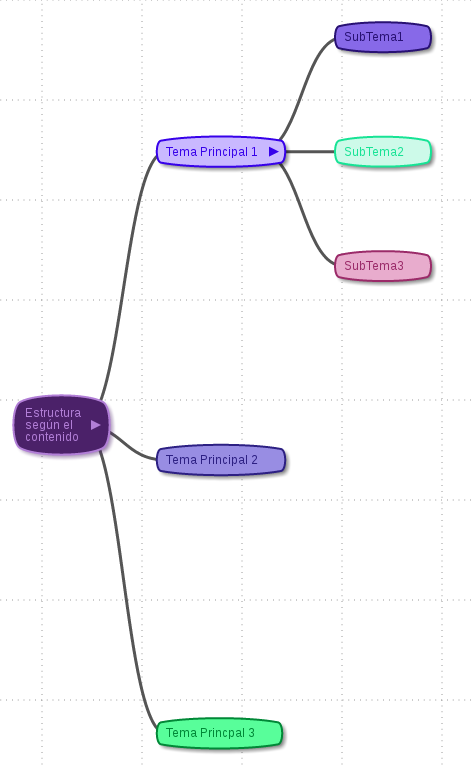
\includegraphics[width=0.6\textwidth]{imagenes/Estructura1.png}
\caption{Partes de un mapa mental considerando su contenido}
\label{fig:partescontenido}
\end{figure}
\section{Elaboración.}

La elaboración de un mapa mental es un gesto sencillo y casi intuitivo, sólo necesitamos partir de una idea central, de la cual vamos ramificando asociando o interconectando símbolos, palabras, tareas o dibujos. 

\begin{figure}[htbp]
\centering
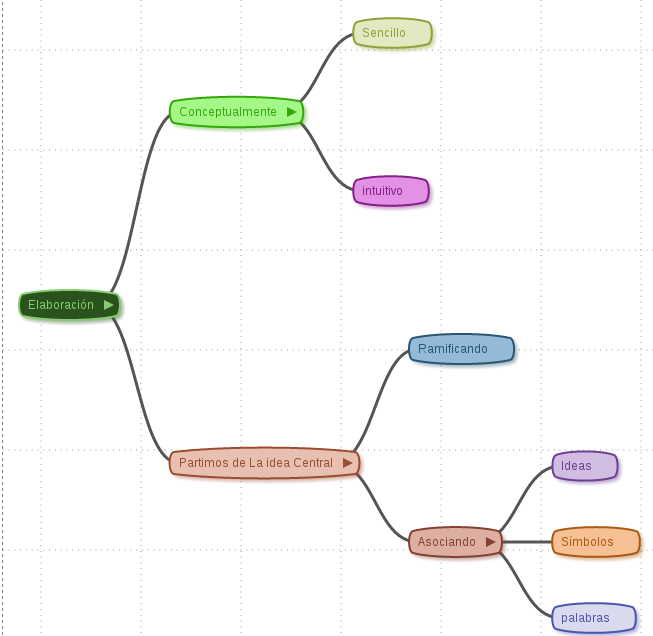
\includegraphics[width=0.7\textwidth]{imagenes/Elaboracion.png}
\caption{Mapa mental de elaboración de mapas mentales}
\label{fig:elaboracion}
\end{figure}

En definitiva, se trata de un diagrama radial que permite a una persona, o grupo de ellas,  plasmar su percepción sobre un tema, o idea, mediante la asociación de conceptos palabras y/o imágenes.



\newpage\mbox{}\thispagestyle{empty}

\chapter{Materiales y métodos}

%En Materiales y métodos se describen los pasos seguidos, las herramientas usadas, 
%también el tiempo y orden del desarrollo. Exponer lo adecuado al trabajo de la 
%metodología empleada así como los métodos en sí para su posible reproducibilidad.



\section{Metodología y etapas del desarrollo.}

\subsection{Metodología de desarrollo ágil.}

En 2001, de un reunión celebrada en EEUU por 17 expertos en la industria del software nace el término “ágil” aplicado al desarrollo de software. El propósito de estos expertos era la elaboración de un manifiesto y principios que permiten a los equipos, a desarrollar software rápidamente y responder a los cambios que surjan a lo largo del proyecto. The Agile Alliance, organización surgida de esta reunión, se dedica a promover los conceptos relacionados con el desarrollo ágil y cómo punto de partida tiene un manifiesto con los siguientes 4 puntos:

\begin{itemize}
\item Individuos e interacciones sobre procesos y herramientas
\item Software funcionando sobre documentación extensiva
\item Colaboración con el cliente sobre negociación contractual
\item Respuesta ante el cambio sobre seguir un plan
\end{itemize}

Quizás estemos ante una de las metodologías de desarrollo más importantes del momento. Se trata de un modelo desarrollo iterativo e incremental donde en cada iteración se elabora una nueva versión para el  usuario final.

El modelo de desarrollo Ágil tiene como principal objetivo la satisfacción del cliente y la elaboración de un software de calidad. Para ello, involucra al usuario en todas las etapas del desarrollo, aportando ideas y realizando pruebas de los productos de cada iteración. El usuario consigue así un software adaptado a sus necesidades, quedando completamente satisfecho del producto final. Con esta estrecha colaboración entre usuario final y el equipo de desarrollo se busca  aunar esfuerzos en pos de un objetivo común.

En cada ciclo se pretende minimizar los riesgos. Es por ello que, para cada iteración se incorpora un conjunto reducidos de funcionalidades. Buscando, no sólo minimizar el riesgo intrínseco al desarrollo, sino que los ciclos de desarrollo sean cortos y se dinamice el proceso productivo. A este respecto, y según los principios de la metodología Ágil, es preferible una  versión incompleta a una con errores.  

Otro aspecto importante, es que la solución y los requerimientos evolucionan de forma continua. Provocando en ocasiones cambios profundos en los diseños preliminares, algo inconcebible en las metodologías clásicas. La refactorización de código se convierte en algo habitual y deseable, si ello nos lleva a una mejor solución.

Un ciclo de desarrollo en la metodología Ágil consta de la siguientes fases:

\begin{itemize}
\item Planificación.
\item Análisis de requerimientos.
\item Diseño.
\item Codificación.
\item Revisión.
\item Documentación.
\end{itemize}

La metodología Ágil se adapta muy bien al desarrollo web. Por esto, y por las características que presenta este paradigma, el proyecto seguirá este modelo de desarrollo.

\subsection{Etapas del desarrollo.}

Viendo la dependencia entre librerías a implementar, lo más apropiado, es seguir un diseño ascendente (bottom-up). Siempre que el estadio anterior haya sido verificado y comprobado su completud, se podrá afrontar con éxito la siguiente etapa. Dicho de otra forma, cada etapa es dependiente de la etapa inmediatamente anterior. Siempre siguiendo la metodología ágil se ha decidido afrontar el proyecto en tres fases o iteraciones:

\textbf{Primera iteración:} se encargará de llevar a buen término la implementación de las librerías Javascripts necesarias para la aplicación. En cada ciclo tendremos que realizar una planificación, análisis de riesgos, implementación, pruebas unitarias y documentación de cada librería. La primera fase constará pues, de seis ciclos bien definidos. El orden de los ciclos es el que sigue:

\begin{figure}[tbph]
\centering
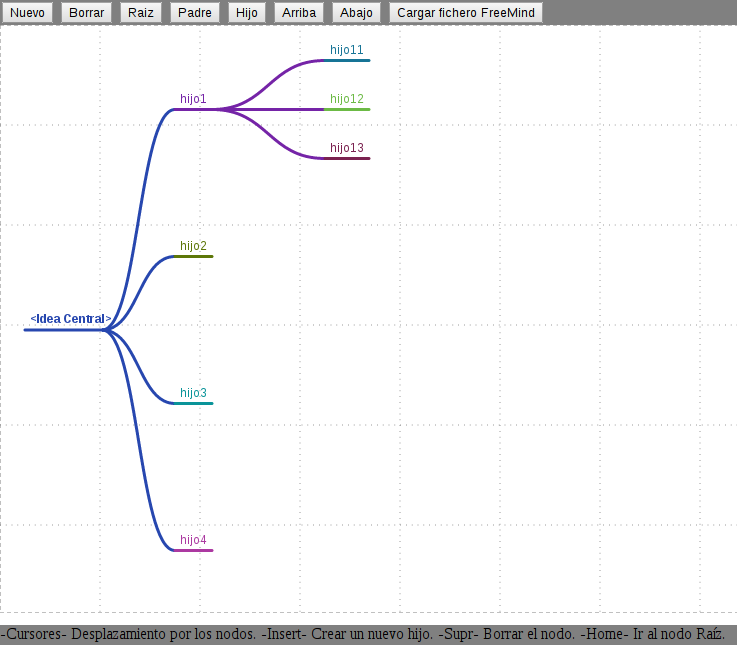
\includegraphics[width=0.5\linewidth]{imagenes/primeraVersion1}
\caption{Versión inicial.}
\label{fig:versioninicial1}
\end{figure}


\begin{itemize}
\item \textbf{Librería base con soporte para herencia.} Esta librería debe tener toda la funcionalidad básica (bindings, curryings, etc) y debe estar muy optimizada ya que el perfecto funcionamiento de la aplicación dependerá en buena medida de ella.

\item \textbf{Librería para manejo de árboles n-arios.} 

\item \textbf{Librería para el manejo de ficheros.} Será la encargada de manejar ficheros, a partir de ella, realizaremos las clases de exportación e importación de mapas mentales de la aplicación. 

\item \textbf{Librería gráfica.} Ciñéndonos al contexto 2D, necesitamos un wrapper sobre la librerías propias del canvas. Esta librería, nos debe permitir pintar, cada uno de los elementos de nuestro árbol. Además de configurar, atributos visuales tales como color del trazo, relleno, etc. No se descarta el uso de alguna librería estándar. Para ello, se realizará una pruebas de concepto sobre ellas.

\item \textbf{Librería para el manejo de eventos del canvas.} El canvas debe reaccionar tanto al teclado, ratón y touch. El canvas viene desprovisto de eventos sobre los elementos pintados en él y es aquí donde entra en juego esta librería. 

\item Por último, las librerías propias del mapa y \textbf{prototipo} o primera versión. 
\end{itemize}

\begin{figure}[tbph]
\centering
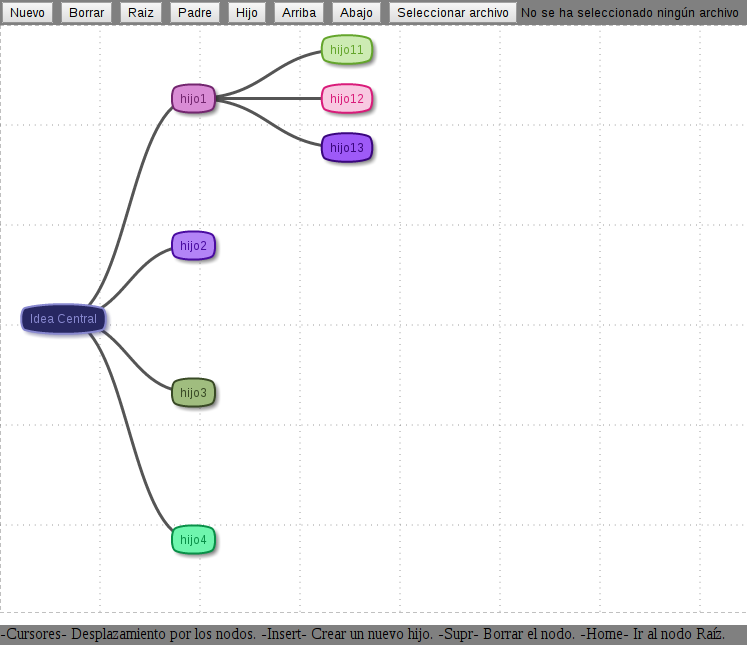
\includegraphics[width=0.5\linewidth]{imagenes/primeraVersion2}
\caption{Versión inicial.}
\label{fig:versioninicial2}
\end{figure}


\textbf{Segunda iteración:} una vez implementadas todas las librerías necesarias y una primera versión (inoperativa), nos encontramos en disposición de ir elaborando la aplicación. Revisión de aspectos visuales de la aplicación tales, como un editor ajustable, zoom, y mejoras en el funcionamiento en general. 

\textbf{Tercera iteración:} nuevas funcionalidades como plegado, hacer-deshacer y un mejor ajuste del en la redistribución de nodos y escalado.



\section{Casos de uso.}

En la figura \ref{fig:casosdeuso} podemos ver de forma general el diagrama de casos de usos.

\begin{figure}[htbp]
\centering
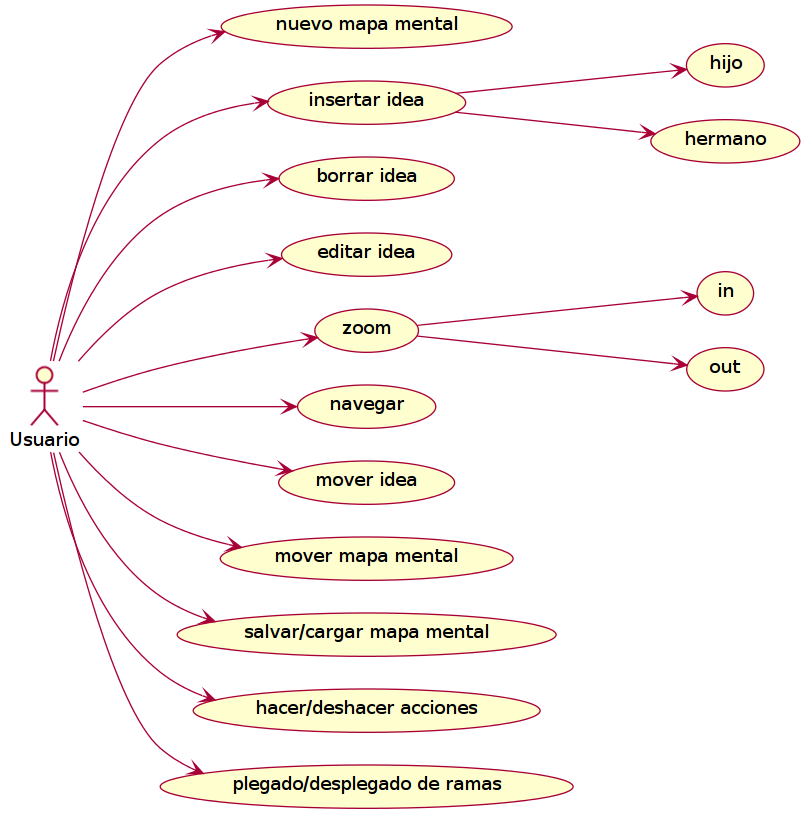
\includegraphics[width=\textwidth]{imagenes/casos-de-uso}
\caption{Casos de uso}
\label{fig:casosdeuso}
\end{figure}

\subsection{Nuevo mapa mental}
El usuario debe de poder reiniciar el editor y empezar un nuevo mapa en cualquier momento. El sistema deberá limpiar la zona de edición eliminando cualquier resto de ediciones anteriores. Una vez borrado se presentará una idea central por defecto que el usuario podrá modificar en todo momento. 

Las acciones que desencadenará esta funcionalidad será un botón y/o la secuencia de teclas $<$Shift+n$>$.

\subsection{Insertar idea}
Mediante el uso de teclado o ratón el usuario podrá crear nuevas ideas. Esta nueva idea podrá ser tanto hija como hermana de la idea actualmente seleccionada. Debe quedar distribuida en función de los nodos existentes en el mapa mental. 

La secuencia de teclados designadas para la creación de ideas. Son $<$ins$>$ para ideas hijas y $<$Shift+Enter$>$ para crear una idea hermana. 

\subsection{Borrar idea}
Con el teclado ($<$supr$>$) y/o ratón el usuario siempre podrá eliminar un idea del mapa mental. Si existen otras ideas que dependan de la idea a borrar estas también se borrarán. Los nodos se redistribuirán en función de los nodos restantes el mapa mental. 

\subsection{Editar idea}
Toda idea será editable en cualquier momento. El usuario podrá activar el modo de edición y modificar el contenido. Se accederá al modo de edición cuando insertemos, naveguemos, o establezcamos el modo de edición. 

Para entrar y salir del modo de edición se utilizarán las teclas $<$Enter$>$ y $<$Esc$>$ respectivamente. Una vez en modo de edición la secuencias de teclas de la aplicación se ajustarán para que $<$Enter$>$ y $<$Tab$>$ permita salir del modo de edición, con $<$Shift+Enter$>$ se inserte un salto de línea y deshabilite el resto de atajos de teclado. El doble clic y doble touch permitirá entrar en modo de edición.

El editor deberá y ajustándose al tamaño del texto insertado.   

\subsection{Zoom}
La aplicación permitirá acciones de zoom o cambio de escala a la imagen. Ampliar ($<$Ctrl++$>$), reducir ($<$Ctrl+-$>$) y reiniciar ($<$Ctrl+0$>$) la escala. Con esta funcionalidad el usuario podrá ajustar las dimensiones del mapa mental a sus necesidades. La rueda del ratón es también una buena opción para realizar zoom in / out.

\subsection{Navegar}
El usuario debe poder moverse por el mapa mental tanto por teclado como con el ratón o touch. El mapa siempre tendrá una idea activa, o focalizada, que podrá variarse mediante un clic, touch o las siguientes secuencias de tecla:

\begin{itemize}
\item Para ir a la \textbf{idea central} $<$home$>$
\item Para ir a la \textbf{idea padre} de la idea actual $<$left$>$
\item Para ir a la \textbf{idea hija} $<$right$>$
\item Para ir a una \textbf{idea hermana} $<$up$>$ y $<$down$>$
\item Para \textbf{navegar por niveles} podemos utilizar $<$tab$>$
\end{itemize}

\subsection{Mover idea}
Con el ratón y touch podremos ajustar la posición de los nodos.

\subsection{Mover mapa mental}
Con el ratón y touch podremos desplazar el mapa.

\subsection{Salvar/cargar mapa mental}
El usuario siempre tendrá opción de salvar y cargar mapas mentales en formato FreeMind. 

\subsection{Hacer/deshacer acciones}
El sistema dispondrá de opciones típicas de edición como hacer y deshacer.

\subsection{Plegado/desplegado de ramas}
Las distintas ideas se podrá plegar o desplegar para una mejor visualización. El sistema deberá ajustar las posiciones de las ideas visibles ( que no estén plegada ) al campo de visión siempre que sea posible. 

Para mayor agilidad el programa dispondrá de una secuencia de teclado para plegar ($<$Shift+-$>$) y desplegar ($<$Shift++$>$) además de botones. 


\section{Diagramas de Clase}

Los diagramas de clases están ordenados por importancia y bloque funcional, siguiendo una
perspectiva bottom-up siempre que sea posible.


\subsubsection{Clase MM.Class}
Como centro de todo el sistema de clases implementado está el MM.Class. Una abstracción del 
patrón constructor que es eje de todas las clases implementadas en la aplicación. A partir 
de ahora, cuando hable de clase me refiero a la herencia efectuada con MM.Class.

La implementación de este objeto es fundamental ya que Javascripts es un lenguaje orientado 
a objetos puro y libre de clases. 

\begin{figure}[tbph]
\centering
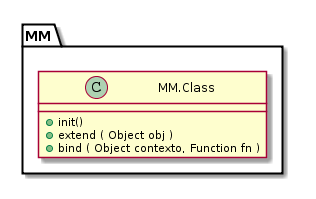
\includegraphics[width=0.4\linewidth]{imagenes/diagrama-clase-mm-class}
\caption{Clase MM.Class}
\label{fig:diagrama-clase-mm-class}
\end{figure}
Los principales métodos son:
\begin{itemize}
\item \textbf{MM.Class.extend:} método que nos permite extender sobre una clase existente.
\item \textbf{MM.Class.init:} Constructor para las clases.
\end{itemize}

Cualquier método sobrescrito dispone en su clase una propiedad \underline{ }super que hace referencia al método sobrescrito, de forma
podamos realizar una llamada al super (o padre).


\subsection{Diagrama de clases PubSub}

Como núcleo de la comunicación entre clases y distintos bloques funcionales, están los eventos. Para ello, se ha desarrollado
la clase MM.PubSub que implementa el patrón Publicador-Suscriptor\footnote{También conocido como patrón Observador-observable}.

\begin{figure}[tbph]
\centering
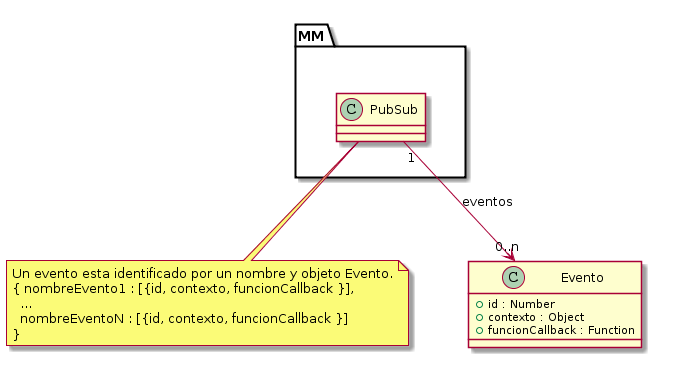
\includegraphics[width=\linewidth]{imagenes/diagrama-clases-mm-pubsub}
\caption{Diagrama de clases pubsub}
\label{fig:diagrama-clases-mm-pubsub}
\end{figure}


El concepto es sencillo, el objeto suscriptor se suscribe a un evento o mensaje concreto y el publicador anuncia a todos los 
suscriptores cuando está lista la suscripción. Un símil muy utilizado, y directo, es el de los suscriptores de un periódico, 
en el cual un lector (o suscriptor) paga un precio para recibir el periódico y la editorial (o publicador) le envía un ejemplar 
cuando lo tiene disponible. 


Los eventos suscritos se registran con un nombre en una lista, que contiene un identificador de suscripción, el contexto de 
ejecución y la función a ejecutar en el momento de la publicación del evento.

\subsubsection{MM.PubSub}
\begin{figure}[tbph]
\centering
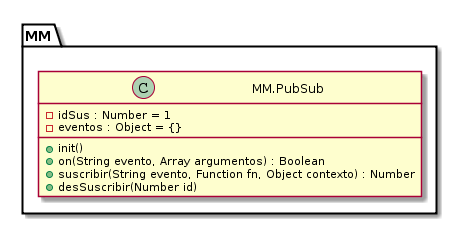
\includegraphics[width=0.5\linewidth]{imagenes/diagrama-clase-mm-pubsub}
\caption{Clase MM.PubSub}
\label{fig:diagrama-clase-mm-pubsub}
\end{figure}

Métodos:
\begin{itemize}
\item \textbf{MM.PubSub.suscribir:} permite a los suscriptores la suscripción a un evento o publicación.
\item \textbf{MM.PubSub.desSuscribir:} permite a los suscriptores la desuscribirse de un evento o publicación.
\item \textbf{MM.PubSub.on:} método que permite al publicador notificar a los suscriptores
la ocurrencia de un evento. 
\end{itemize}





\subsection{Diagrama de clases MM.UndoManager}

Dentro de la edición, otro punto importante son las funciones de hacer y deshacer. Para ello, se ha implementado un manejador que se encarga de registrar, en una lista de comandos, los cambios 
realizados en el editor.

\begin{figure}[tbph]
\centering
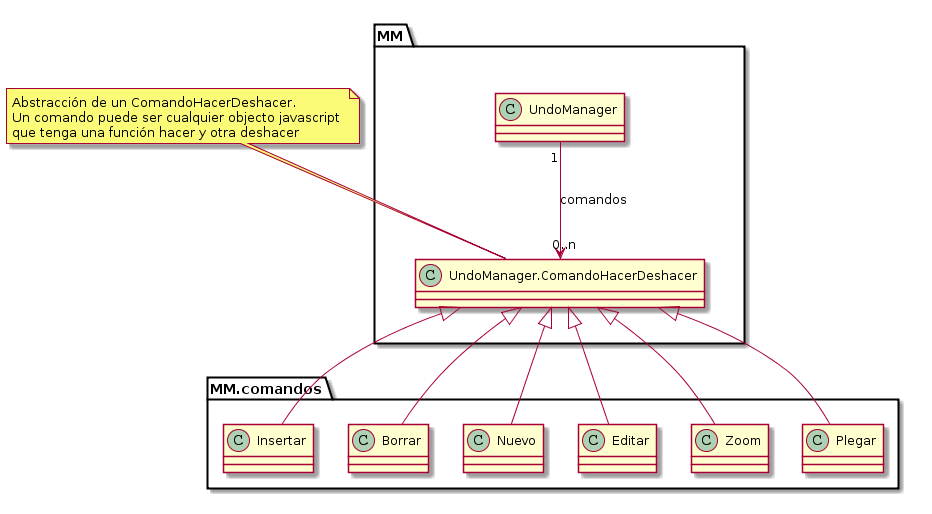
\includegraphics[width=\linewidth]{imagenes/diagrama-clases-mm-undo}
\caption{Diagrama de clases undo}
\label{fig:diagrama-clases-mm-undo}
\end{figure}

\subsubsection{Clase MM.UndoManager.ComandoHacerDeshacer}

La clase MM.UndoMangerComandoHacerDeshacer es la clase base para todos los comandos para hacer y
deshacer del editor de mapas mentales. De ella, como se puede observar en la figura \ref{fig:diagrama-clases-mm-undo}, heredan clases para hacer y deshacer inserciones, borrados, 
zoom, etc ...  

\begin{figure}[tbph]
\centering
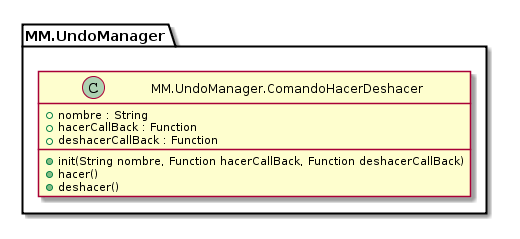
\includegraphics[width=0.7\linewidth]{imagenes/diagrama-clase-mm-undomanager-comandohacerdeshacer}
\caption{Clase MM.UndoManager.ComandoHacerDeshacer}
\label{fig:diagrama-clase-mm-undomanager-comandohacerdeshacer}
\end{figure}

Todo comando deberá tener un nombre e implementar los métodos hacer y deshacer. La funcionalidad del 
método hacer se encargará de repetir la operación ejecutada y el deshacer de revertir la.

\subsubsection{Clase MM.UndoManager}

El manejador de acciones hacer/deshacer tiene un registro de comandos ejecutados en la aplicación y un puntero\footnote{Campo actual.} que indica el último comando ejecutado. El funcionamiento consiste en que siempre se pueda deshacer la última acción ejecutada, apuntada por el puntero actual, y sólo se pueda hacer el comando siguiente al puntero actual.

\begin{figure}[tbph]
\centering
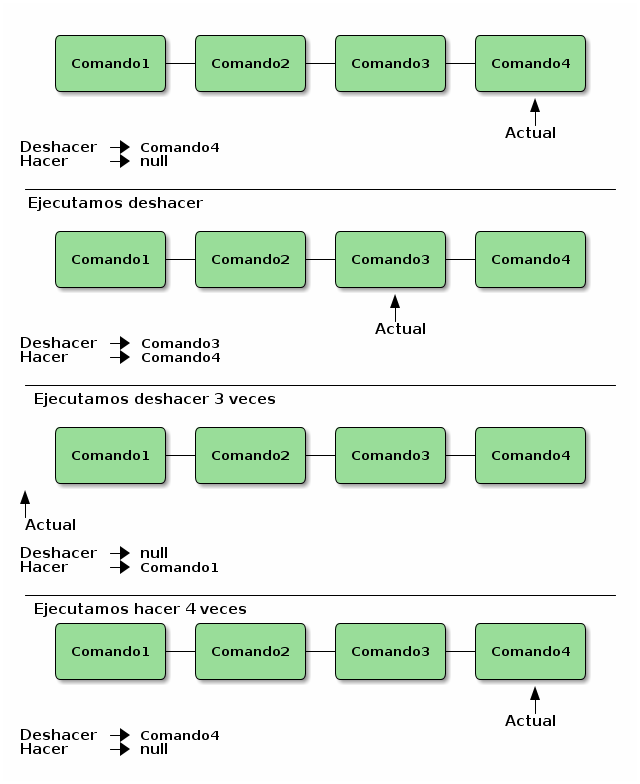
\includegraphics[width=0.7\linewidth]{imagenes/undomangerEjecucion.png}
\caption{Secuencia de ejecución de UndoManager}
\label{fig:undomanager-ejecucion-concepto}
\end{figure}
 
Como puede observar en la figura \ref{fig:undomanager-ejecucion-concepto} el puntero \textit{Actual} indica que comando se puede deshacer y \textit{Actual + 1} el comando que se puede hacer. 

\begin{figure}[tbph]
\centering
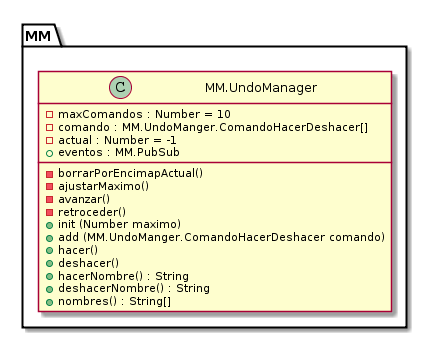
\includegraphics[width=0.7\linewidth]{imagenes/diagrama-clase-mm-undomanager}
\caption{Clase MM.UndoManager}
\label{fig:diagrama-clase-mm-undomanager}
\end{figure}

Los métodos:
\begin{itemize}
\item \textbf{MM.UndoManager.init:} al constructor se le puede indicar el máximo de la pila 
de ejecución.
\item \textbf{MM.UndoManager.add:} añade un nuevo comando a la pila de ejecución.
\item \textbf{MM.UndoManager.hacer:} ejecuta el hacer del comando que apunta actual + 1 y avanza 
el puntero. 
\item \textbf{MM.UndoManager.deshacer:} ejecuta el deshacer del comando que apunta actual y 
retrocede el puntero.
\item \textbf{MM.UndoManager.hacerNombre:} devuelve el nombre del siguiente comando hacer.
\item \textbf{MM.UndoManager.deshacerNombre:} devuelve el nombre del siguiente comando deshacer.
\item \textbf{MM.UndoManager.nombres:} lista de comandos en la lista.
\end{itemize}






\subsection{Diagrama de clases MM}

El centro de la aplicación es sin lugar a dudas el módulo MM. El módulo MM aglutina y vertebra la 
ejecución del editor de mapas mentales. 

\begin{figure}[tbph]
\centering
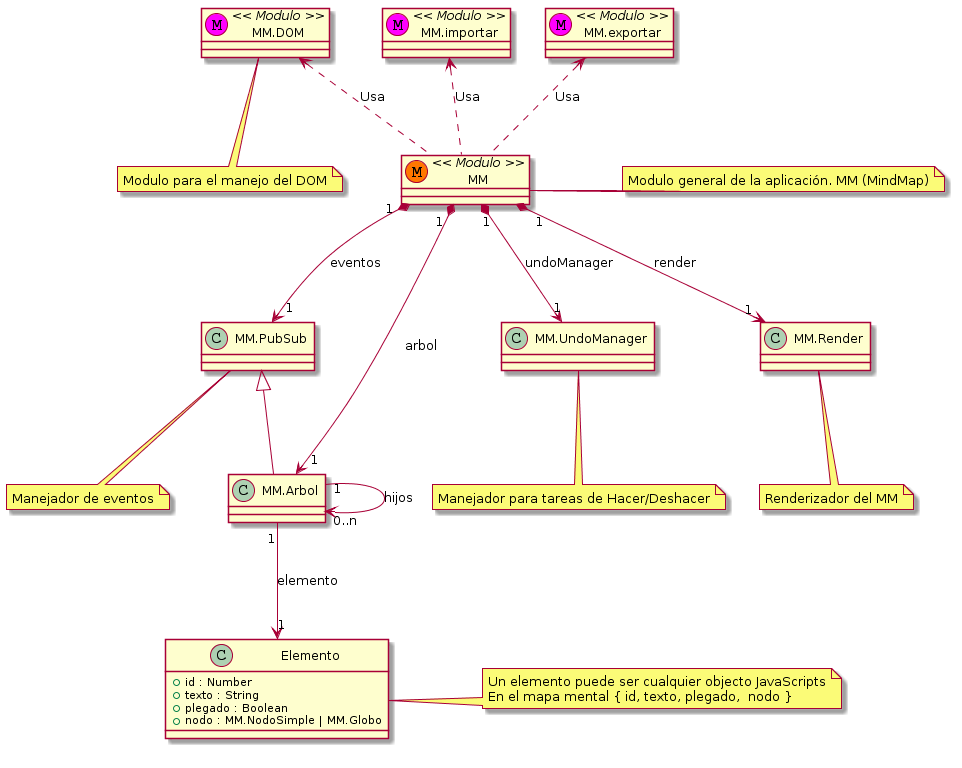
\includegraphics[width=\linewidth]{imagenes/diagrama-clases-mm}
\caption{Diagrama de clases MM}
\label{fig:diagrama-clases-mm}
\end{figure}

Una mapa Mental (MM) tiene un árbol que representa la estructura del mapa mental y un manejador de 
eventos con el que podemos publicar los eventos de la aplicación para avisar a otras partes integrantes del sistema\footnote{Por ejemplo al render o al interface de usuario}. Así pues cuando el usuario añade un añade un nuevo elemento al mapa mental, MM se encargará:

\begin{itemize}
\item Mantener la coherencia de los datos.
\item Registrar el comando ejecutado en el UndoManager
\item Y avisar o publicar el evento de para indicar la operación realizada.
\end{itemize}

Cada elemento de un nodo del árbol tiene un id de nodo, un texto, un indicador de plegado y un nodo gráfico.

\subsubsection{Módulo MM}

\begin{figure}[tbph]
\centering
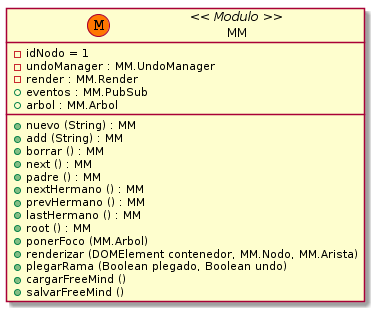
\includegraphics[width=0.5\linewidth]{imagenes/diagrama-clase-mm}
\caption{Clase MM}
\label{fig:diagrama-clase-mm}
\end{figure}

El módulo tiene los siguientes métodos:
\begin{itemize}
\item \textbf{MM.nuevo:} crea un nuevo mapa mental.
\item \textbf{MM.add:} añade un nuevo nodo hijo al nodo activo.
\item \textbf{MM.borrar:} borra el nodo activo.
\item \textbf{MM.next:} mueve el foco al primer hijo del nodo activo.
\item \textbf{MM.padre:} mueve el foco al padre del nodo activo.
\item \textbf{MM.nextHermano:} mueve el foco al siguiente hermano del nodo activo.
\item \textbf{MM.prevHermano:} mueve el foco al hermano anterior del nodo activo.
\item \textbf{MM.lastHermano:} mueve el foco al último hermano del nodo activo.
\item \textbf{MM.root:} mueve el foco al nodo raíz.
\item \textbf{MM.ponerFoco:} establece el foco en nodo dado.
\item \textbf{MM.renderizar:} se encarga de renderizar el mapa mental.
\item \textbf{MM.plegarRama:} función para plegar y desplegar ramas.
\item \textbf{MM.cargarFreeMind:} función de carga de ficheros FreeMind.
\item \textbf{MM.salvarFreeMind:} se encarga de salvar el mapa mental en formato FreeMind.
\end{itemize}



\subsubsection{Clase MM.Arbol}

\begin{figure}[tbph]
\centering
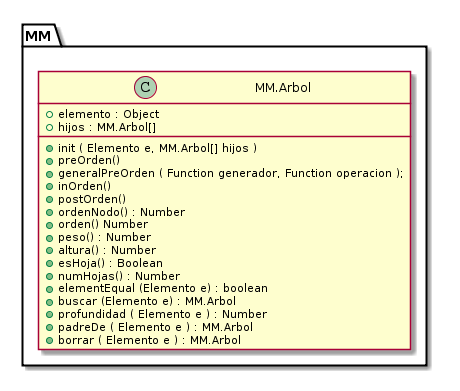
\includegraphics[width=0.7\linewidth]{imagenes/diagrama-clase-mm-arbol}
\caption{Clase MM.Arbol}
\label{fig:diagrama-clase-mm-arbol}
\end{figure}

La implementación MM.Arbol debe ser una implementación funcional de un árbol-n lo más general posible. 

\begin{itemize}
\item \textbf{MM.Arbol.init:} Crea un nuevo árbol-n con un elemento raíz y array de árboles hijos.
\item \textbf{MM.Arbol.preOrden:} realiza un recorrido en preorden por el árbol.
\item \textbf{MM.Arbol.generalPreOrden:} recorrido en preorden, con un generador que trata el elemento actual y una operación que se encarga de operar el elemento generado con el preorden de los nodos hijos.
\item \textbf{MM.Arbol.inOrden:} realiza un recorrido inorden por los elementos del árbol.
\item \textbf{MM.Arbol.postOrden:} recorre el árbol el postorden.
\item \textbf{MM.Arbol.ordenNodo:} calcula el orden del nodo actual.
\item \textbf{MM.Arbol.orden:} calcula el orden del árbol completo.
\item \textbf{MM.Arbol.peso:} calcula el peso de un árbol.
\item \textbf{MM.Arbol.altura:} altura del árbol.
\item \textbf{MM.Arbol.esHoja:} indica si el nodo actual es un nodo hoja o no.
\item \textbf{MM.Arbol.numHojas:} determina el número de nodos hojas del árbol.
\item \textbf{MM.Arbol.elementEqual:} función de igual entre elementos de los nodos. Por defecto, es la igual estricta '==='. Esta función podrá ser sobreescrita para adecuarse al tipo de elemento guardado en cada nodo.
\item \textbf{MM.Arbol.buscar:} busca un elemento en el árbol. Como comparador de nodos se utiliza la función MM.Arbol.elementEqual.
\item \textbf{MM.Arbol.profundidad:} determina la profundidad del árbol.
\item \textbf{MM.Arbol.padreDe:} calcula el árbol padre del elemento pasado.
\item \textbf{MM.Arbol.borrar:} borra un elemento del árbol.
\end{itemize}



\subsubsection{Módulo MM.DOM}

El módulo MM.DOM contendrá funciones para el manejo del DOM. Creación y borrado de elementos DOM. 

\begin{figure}[tbph]
\centering
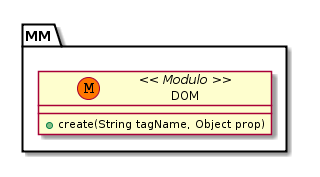
\includegraphics[width=0.4\linewidth]{imagenes/diagrama-clase-mm-dom}
\caption{Modulo MM.DOM}

\label{fig:diagrama-clase-mm-dom}
\end{figure}



\subsubsection{Clase MM.Render}

La clase MM.Render es la encargada de pintar el mapa mental y realizar los ajustes visuales necesarios para mostrar los nodos y las aristas. El renderizador se configura o inicializa entorno a un elemento DOM, normalmente un \textit{div}, una clase que MM.NodoSimple\footnote{O que herede de MM.NodoSimple como MM.Globo} y una clase MM.Arista\footnote{O que herede de MM.Arista}. A partir de estos datos el sistema es capaz de ir generando el mapa mental en función de los eventos producidos en el módulo MM. 

\begin{figure}[tbph]
\centering
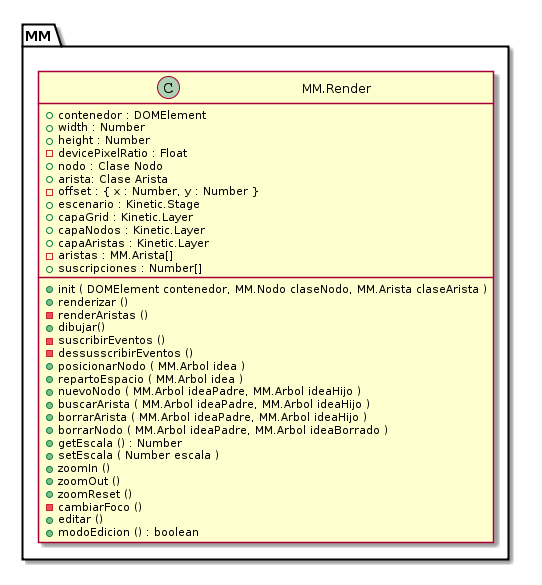
\includegraphics[width=0.65\linewidth]{imagenes/diagrama-clase-mm-render}
\caption{Modulo MM.Render}

\label{fig:diagrama-clase-mm-render}
\end{figure}

La clase MM.Render dispone de los siguientes métodos: 
\begin{itemize}
\item \textbf{MM.Render.init:} constructor de la clase render. Inicializa las capas de nodos y aristas. 
\item \textbf{MM.Render.renderizar:} se encarga de realizar las suscripciones a eventos, dibujar y establecer los atajos de teclado.
\item \textbf{MM.Render.renderizarAristas:} pinta las aristas entre los distintos nodos.
\item \textbf{MM.Render.dibubar:} en función del mapa actual del módulo MM dibuja y reparte el espacio de dibujo.
\item \textbf{MM.Render.suscribirEventos / dessuscribirEventos:} métodos de activar y desactivar las suscripciones a eventos del render.  
\item \textbf{MM.Render.get/setEscala:} establece o devuelve la escala actual.
\item \textbf{MM.Render.zoomIn / zoomOut / zoomReset :} funciones de zoom, en orden, aumenta, disminuye o reinicia la escala del mapa mental.
\item \textbf{MM.Render.cambiarFoco:} se encarga de resalta la idea que tiene el foco actual.
\item \textbf{MM.Render.modoEdicion:} indica si la idea actual esta en modo de edición o no.
\item \textbf{MM.Render.editar:} establece la idea actual en modo de edición. Mostrando el editor del nodo y activando y desactivando atajos de teclados y eventos.
\item \textbf{MM.Render.nuevoNodo:} manejador de eventos para cuando se inserta una nueva idea. Se encarga de insertar la nueva idea y enlazar la idea padre con la hija mediante una arista. El sistema de establece la mejor ubicación para el nuevo elemento.
\item \textbf{MM.Render.borrarNodo:} manejador de eventos para cuando se borra un idea y la correspondiente arista. Además se debe redistribuir el mapa mental en función de los nodos restantes.
\item \textbf{MM.Render.buscarArista:} busca una arista entre dos ideas.
\item \textbf{MM.Render.borrarArista:} borra una arista existente entre dos ideas.
\end{itemize}



\subsection{Diagrama de clases nodo.}
El nodo se encarga del pintado de una idea del mapa mental, en esencia, es un MM.Mensaje al cual se le han añadido otros elementos gráficos y funcionalidades. Existen dos implementaciones de nodo, como se pueden ver en el diagrama\ref{fig:diagrama-clases-mm-render}, el MM.NodoSimple y el MM.Globo, y ambos pueden ser usados desde MM.Render. Todos los nodos existen en un escenario y en una capa dada. 

\begin{figure}[tbph]
\centering
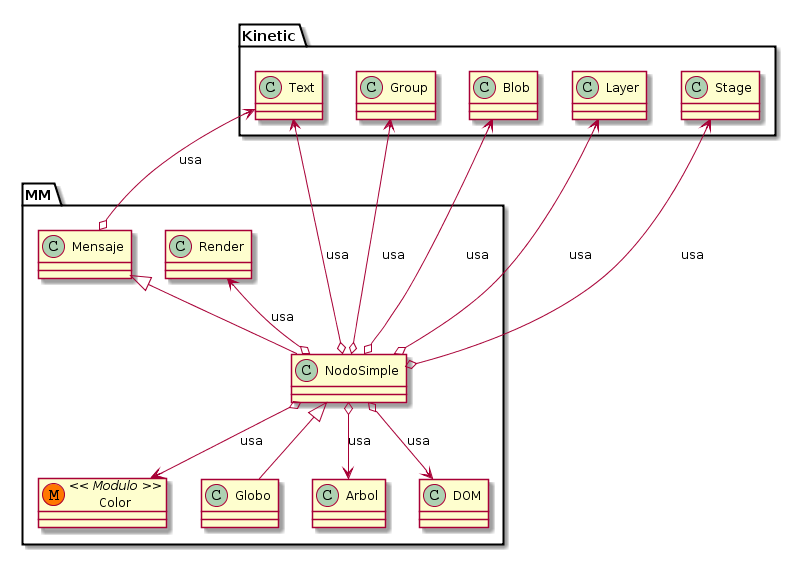
\includegraphics[width=\linewidth]{imagenes/diagrama-clases-mm-render}
\caption{Diagrama de clases nodo}
\label{fig:diagrama-clases-mm-render}
\end{figure}


\subsubsection{Clase MM.Mensaje.}
Se trata de una simple clase que pinta un texto en una capa dada. 

\begin{figure}[tbph]
\centering
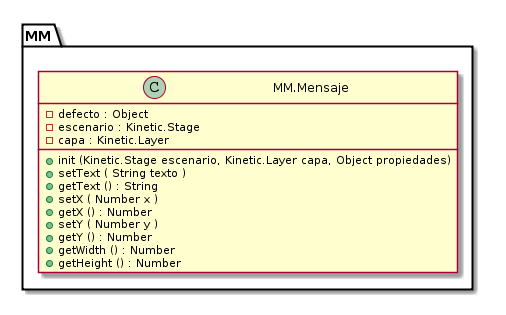
\includegraphics[width=0.7\linewidth]{imagenes/diagrama-clase-mm-mensaje}
\caption{Clase MM.Mensaje}
\label{fig:diagrama-clase-mm-mensaje}
\end{figure}

\begin{itemize}
\item \textbf{MM.Mensaje.init:} constructor de la clase. Tiene el escenario y la capa donde pintar el mensaje, además de un objeto de propiedades con la posición, texto, etc...
\item \textbf{MM.Mensaje.getText/setText:} métodos para establecer y obtener el texto del mensaje. 
\item \textbf{MM.Mensaje.getX/setX:} métodos para establecer y obtener la posición\footnote{en píxeles} X del mensaje.
\item \textbf{MM.Mensaje.getY/setY:} métodos para establecer y obtener la posición Y\footnote{en píxeles} del mensaje.
\item \textbf{MM.Mensaje.getWidth:} devuelve el ancho del texto en píxeles.
\item \textbf{MM.Mensaje.getHeight:} devuelve el alto del texto en píxeles.
\end{itemize}

\subsubsection{Clase MM.NodoSimple.}
Hereda de MM.Mensaje y representa un mensaje o idea subrayada. El nodo representa una idea que será renderizada y creada desde MM.Render. Su funcionalidad básica pasa por obtener el foco cuando sea la idea activa, poderse editar, ocultar cuando su rama este plegada o mostrar cuando este desplegada.

\begin{figure}[tbph]
\centering
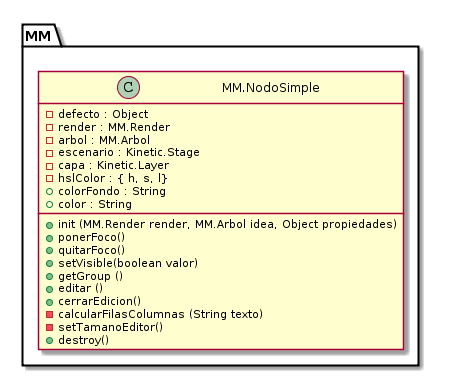
\includegraphics[width=0.6\linewidth]{imagenes/diagrama-clase-mm-nodosimple}
\caption{Clase MM.NodoSimple}
\label{fig:diagrama-clase-mm-nodosimple}
\end{figure}

\begin{figure}[tbph]
\centering
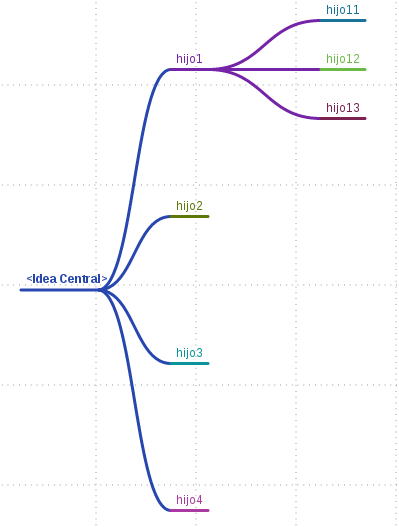
\includegraphics[width=0.5\linewidth]{imagenes/NodoSimple}
\caption{Mapa mental con renderización de nodos simples}
\label{fig:nodosimple}
\end{figure}

\begin{itemize}
\item \textbf{MM.NodoSimple.init:} constructor de la clase. Recibe el MM.Render, la idea a la que representa y un conjunto de propiedades como la posición, escala, etc ...
\item \textbf{MM.ponerFoco/quitarFoco:} métodos que poner o quitan el foco en la idea que representa el nodo. Debe resaltar el nodo cuando este esté focalizado. 
\item \textbf{MM.Mensaje.editar/cerrarEdicion:} métodos para establecer la idea en modo edición y para cerrarlo cuando se termine la edición. Si esta en modo edición debe tener el foco.
\item \textbf{MM.Mensaje.setVisible:} indica si el mensaje debe mostrarse o no.
\item \textbf{MM.Mensaje.destroy:} borra y destruye el nodo.
\end{itemize}


\subsubsection{Clase MM.Globo.}
Se trata de un nodo más elaborado. Representa al texto de la idea incluido en un globo.

\begin{figure}[tbph]
\centering
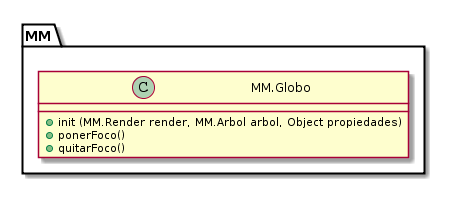
\includegraphics[width=0.6\linewidth]{imagenes/diagrama-clase-mm-globo}
\caption{Clase MM.Globo}
\label{fig:diagrama-clase-mm-globo}
\end{figure}

\begin{figure}[tbph]
\centering
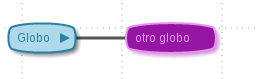
\includegraphics[width=0.3\linewidth]{imagenes/NodoGlobo}
\caption{Mapa mental con renderización de nodos globo}
\label{fig:nodoglobo}
\end{figure}

\subsubsection{Módulo MM.Color.}
Módulo con funcionalidades de color. Permite generar distintos representaciones de color\footnote{HSL, RGB y HUE} y realizar conversiones sobre los distintos tipos. 

\begin{figure}[tbph]
\centering
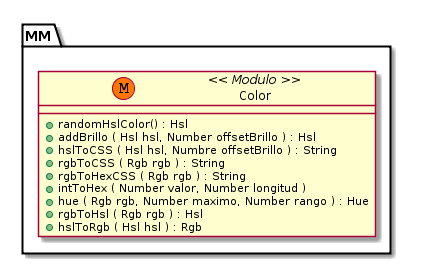
\includegraphics[width=0.5\linewidth]{imagenes/diagrama-clase-mm-color}
\caption{Modulo MM.Color}
\label{fig:diagrama-clase-mm-color}
\end{figure}



\subsection{Diagrama de clases de aristas.}
Una arista representa la línea de unión entre dos ideas o nodos. Existen dos tipos de aristas MM.Arista y MM.Rama, ambas tienen dos nodos a los deben unir. Las aristas, han sido implementadas con una curva Beizer. El diagrama de clases de aristas podemos ver lo en la figura \ref{fig:diagrama-clases-mm-aristas}.

\begin{figure}[tbph]
\centering
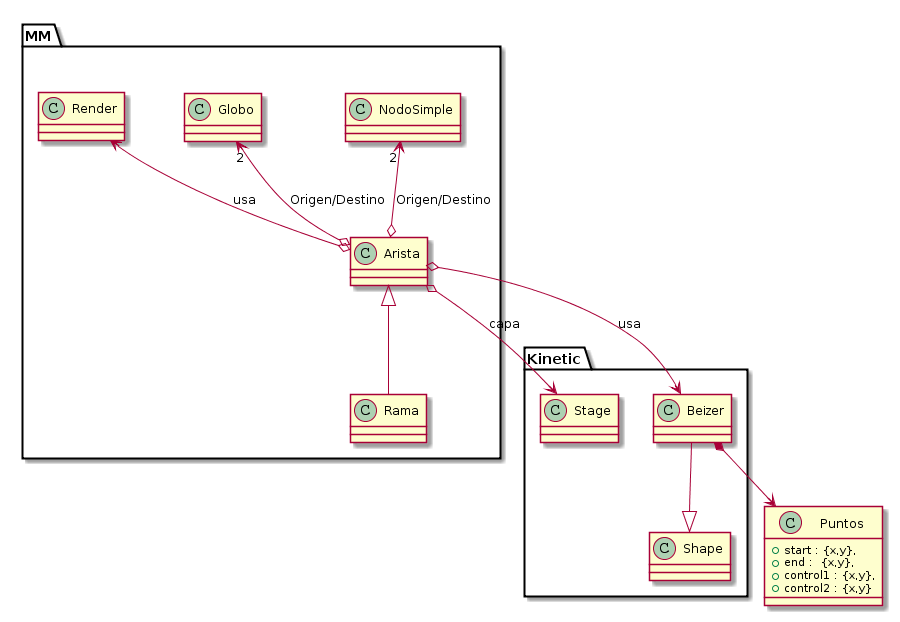
\includegraphics[width=\linewidth]{imagenes/diagrama-clases-mm-aristas}
\caption{Diagrama de clases aristas}
\label{fig:diagrama-clases-mm-aristas}
\end{figure}

\subsection{Clase Kinetic.Beizer.}
Extensión realizada en la librería KineticJS. Una curva Beizer está representada por cuatro puntos inicio, fin y dos puntos de control que determinan la curvatura. En el constructor debe recibir un objeto con los puntos de inicio, fin y de control. Esta clase se encarga de pintar en un canvas la curva en cuestión. 

\begin{figure}[tbph]
\centering
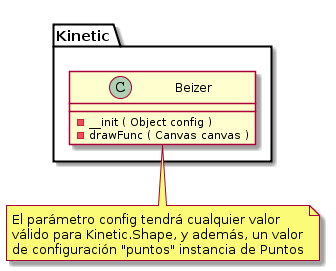
\includegraphics[width=0.5\linewidth]{imagenes/diagrama-clase-kinetic-beizer}
\caption{Clase Kinetic Beizer}
\label{fig:diagrama-clase-kinetic-beizer}
\end{figure}

\subsubsection{Clase MM.Arista.}
Una arista recibe dos ideas y un tamaño (o grosor de línea). Esta clase en cuestión se encarga de unir dos ideas mediante una curva beizer, y de mantenerlos unidos a pesar de los cambios.

\begin{figure}[tbph]
\centering
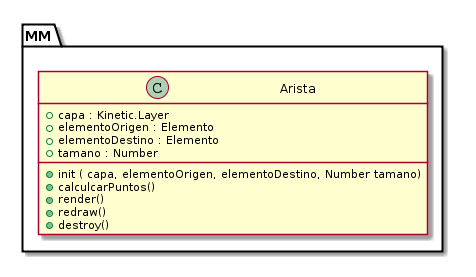
\includegraphics[width=0.7\linewidth]{imagenes/diagrama-clase-mm-arista}
\caption{Clase MM.Arista}
\label{fig:diagrama-clase-mm-arista}
\end{figure}

\begin{itemize}
\item \textbf{MM.Arista.init:} constructor de la clase.
\item \textbf{MM.Arista.calcularPuntos:} calcula los puntos para dibujar la curva.
\item \textbf{MM.Arista.render:} dibuja la curva beizer.
\item \textbf{MM.Arista.rendraw:} redibuja la curva beizer para adaptarse a los cambios producidos en su entorno.
\item \textbf{MM.Arista.destroy:} borra y destruye la arista.
\end{itemize}


\subsubsection{Clase MM.Rama.}
Se trata de otro tipo de arista pensada para unir dos nodos de tipo MM.NodoSimple.

\begin{figure}[tbph]
\centering
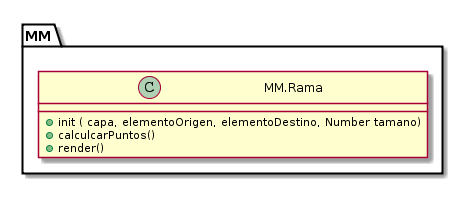
\includegraphics[width=0.7\linewidth]{imagenes/diagrama-clase-mm-rama}
\caption{Clase MM.Rama}
\label{fig:diagrama-clase-mm-rama}
\end{figure}



\subsection{Diagrama de clases de teclado}
Para una mejor experiencia de usuario se ha implementado un complejo manejador de teclados para procesar secuencias de teclas del tipo \textit{Modificadores+tecla}. El manejo de teclado en el mundo web puede complicarse bastante ya que dependen del navegador y el sistema operativo, ya no sólo por que pueden existir o no teclas como \textit{Meta}\footnote{En los sistemas Mac.} o \textit{Windows}, si no por que existen teclas como \textit{+} que tienen distinto keycode en un Firefox, Chrome y Safari.

También hay que tener en cuenta que las aplicaciones web no han sido pensadas para un uso intensivo de teclado.   

\begin{figure}[tbph]
\centering
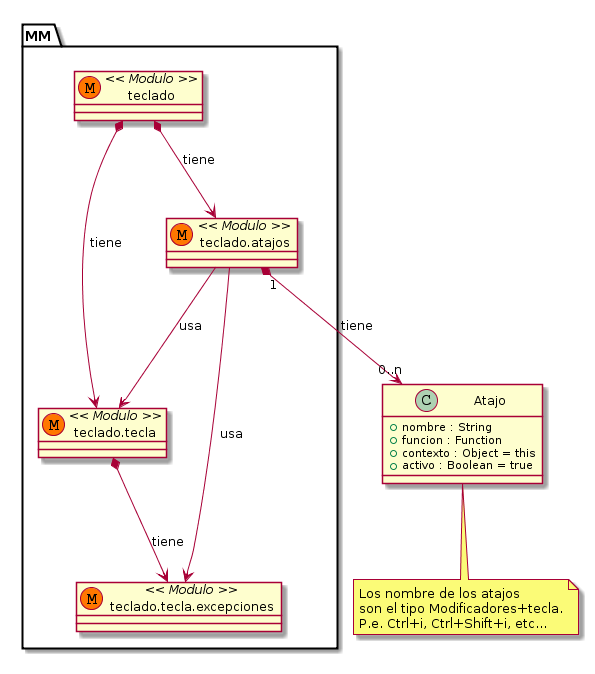
\includegraphics[width=0.8\linewidth]{imagenes/diagrama-clases-mm-teclado}
\caption{Diagrama de clases teclado}
\label{fig:diagrama-clases-mm-teclado}
\end{figure}


\subsubsection{Módulo MM.teclado.atajos}
Un atajo esta compuesto por un nombre\footnote{Ctrl+i}, una función que será ejecutada cuando se
detecte la pulsación de la secuencia de teclas. Un atajo puede estar activado o desactivado, es
decir, que se ejecutará cuando se detecte el atajo de teclado o no. 

El módulo de atajos registrar los atajos de teclados del sistema.


\begin{figure}[tbph]
\centering
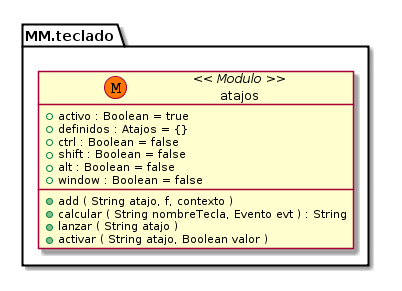
\includegraphics[width=0.6\linewidth]{imagenes/diagrama-clase-mm-teclado-atajos}
\caption{Modulo MM.teclado.atajos}
\label{fig:diagrama-clase-mm-teclado-atajos}
\end{figure}

\begin{itemize}
\item \textbf{MM.teclado.atajos.add:} añade un nuevo atajo de teclado al sistema.
\item \textbf{MM.teclado.atajos.calcular:} calcula el atajo de teclado producido.
\item \textbf{MM.teclado.atajos.lanzar:} lanza un atajo de teclado, es decir, la función asociada. 
\item \textbf{MM.teclado.atajos.activar:} activa o desactiva un atajo de teclado 
\end{itemize}

\subsubsection{Módulo MM.teclado.tecla}
Se trata de un conjunto de constantes de códigos de teclados. También incluye las posibles
excepciones y discordancias que se producen entre los distintos navegadores y sistemas operativos.

\begin{figure}[tbph]
\centering
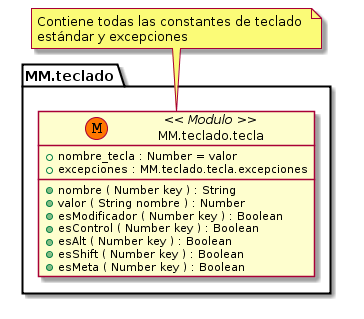
\includegraphics[width=0.4\linewidth]{imagenes/diagrama-clase-mm-teclado-tecla}
\caption{Clase MM.teclado.tecla}
\label{fig:diagrama-clase-mm-teclado-tecla}
\end{figure}

\begin{itemize}
\item \textbf{MM.teclado.tecla.nombre:} calcula el nombre de una tecla en función de su código.
\item \textbf{MM.teclado.tecla.valor:} nos devuelve el código de tecla en función del nombre.
\item \textbf{MM.teclado.tecla.esModificador:} indica si un código de teclado es un modificador. 
\item \textbf{MM.teclado.tecla.esControl:} indica si el código de teclado se corresponde con la tecla $<$Control$>$.
\item \textbf{MM.teclado.tecla.esAlt:} indica si el código de teclado se corresponde con la tecla $<$Alt$>$.
\item \textbf{MM.teclado.tecla.esShift:} indica si el código de teclado se corresponde con la tecla $<$Shift$>$.
\item \textbf{MM.teclado.tecla.esMeta:} indica si el código de teclado se corresponde con la tecla $<$Meta$>$.
\end{itemize}


\subsubsection{Módulo MM.teclado}
Módulo encargado de mantener el registro de atajos y manejar los eventos de teclado.

\begin{figure}[tbph]
\centering
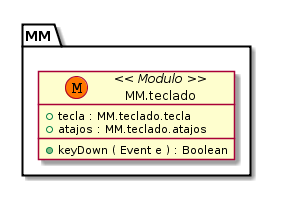
\includegraphics[width=0.4\linewidth]{imagenes/diagrama-clase-mm-teclado}
\caption{Clase MM.teclado}
\label{fig:diagrama-clase-mm-teclado}
\end{figure}

El sistema de control de teclado se encarga de recoger todos los eventos\footnote{Todos los eventos KeyDown del navegador.} de pulsación de teclas y revisar y calcular si se trata de un atajo registrado en el sistema y lanzar la función asociada a dicho atajo.

\begin{figure}[tbph]
\centering
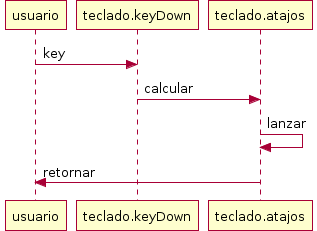
\includegraphics[width=0.4\linewidth]{imagenes/diagrama-seq-teclado}
\caption{Diagrama de secuencia teclado}
\label{fig:diagrama-seq-teclado}
\end{figure}




\newpage\mbox{}\thispagestyle{empty}

\chapter{Implementación.}

La implementación describe los detalles más difíciles, las soluciones elegidas, y 

presenta esquemas y también detalles relevantes de programas, algoritmos y métodos 

de trabajo y tareas de campo desarrollados.
\section{Javascripts.}

\subsection{Qué es.}

Mozilla, los herederos directos de Netscape, definen Javascripts como:\footnote{MDN (Mozilla Developer Network)} \footnote{https://developer.mozilla.org/en-US/docs/Web/JavaScript/Guide/JavaScript\_Overview}

\begin{quotation}
Javascripts is a cross-platform, object-oriented scripting language. JavaScript is a small, lightweight language; it is not useful as a standalone language, but is designed for easy embedding in other products and applications, such as web browsers. Inside a host environment, JavaScript can be connected to the objects of its environment to provide programmatic control over them.
\end{quotation}

Definición que desde mi punto de vista se queda corta. Ya que Javascripts es un lenguaje de scripting (que debe ser interpretado), imperativo, estructurado, orientado a objeto sin clases, débilmente tipado, dinámico, funcional y basado en prototipos.

De C ha heredado que sea un lenguaje imperativo y estructurado con distinción entre sentencias y expresiones. A diferencia de C y Java el ámbito de las variables no son a nivel de bloque sino de función, es decir, que una variable definida dentro de una sentencia puede ser utilizada fuera de dicha sentencia, ya que el ámbito no lo define la sentencia sino la función que la contiene.

\begin{lstlisting}[language=JavaScript, numbers=left]
var f = function (valor) {
	if ( valor ) {
		var resultado = 'Si';
	} 
	return resultado;
};
\end{lstlisting}

Sin lugar a dudas se trata de un lenguaje orientado a objeto. Los arrays, números, funciones, cadenas, casi en su totalidad el lenguaje son objetos\footnote{Salvo los valores destacados null y undefined, el resto de valores Javascripts son objetos}. Los objetos son array asociativos al cual podemos acceder a través de la notación objeto.campo o como si de un array se tratará. 

\begin{lstlisting}[language=JavaScript, numbers=left]
var f = function () {
	var objeto = { 
		campo0 : 0,
		campo1 : 'una cadena' 
	};
	
	var valorCampo0 = objeto.campo0;
	valorCampo0 = objecto['campo0'];
};
\end{lstlisting}

Es débilmente tipado, el tipo no va asociado a la variable si al valor que contiene. Por lo que podemos crear variables y asignarle un valor numérico y posteriormente una cadena. 

\begin{lstlisting}[language=JavaScript, numbers=left]
var f = function () {
	var numero = 1;
	numero++;
	numero = '1';
};
\end{lstlisting}

Se trata de un lenguaje funcional en el que una función es un objeto de primera clase. Esto significa que Javascripts soporta el paso de funciones como argumentos a otras funciones, funciones que devuelve funciones, variables que almacenan funciones, creación de funciones anónimas, etc ...

\begin{lstlisting}[language=JavaScript, numbers=left]
function map(f, xs) {
	var result = new Array();
	for (var i = 0; i < xs.length; i++)
		result.push(f.apply(null, [xs[i]]));
	return result;
}
\end{lstlisting}

Javascripts no utiliza los mecanismos de clases para implementar la herencia, para ello hace uso de los prototipos. 

\begin{lstlisting}[language=JavaScript, numbers=left]
var Persona = function (){
	this.nombre = 'Sin nombre';
};

Persona.prototype.setNombre = function () {
	this.nombre;
};

var pepe = new Persona(); // pepe es una instancia de Persona 
pepe.setNombre('Pepe');   // y contiene una copia del prototipo de Persona.
\end{lstlisting}


\subsection{Un poco de historia.}

Cuando en 1996, el navegador Netscape introdujo su primer interprete de
Javascripts\footnote{Javascripts fue un nombre por conveniencia legal. Originalmente se llamaba
  LiveScript} nadie podía intuir la importancia que adquiriría años después. 

Internet aun estaba en pañales, navegar era lento\footnote{La velocidad máxima de los modems de
  usuario era 28.8Kbps} y los ordenadores personales poco potentes. En el mejor de los casos, el
usuario tenía que esperar durante largo tiempo para poder interactuar con la web solicitada.  Las
páginas comenzaban a ser más complejas, y la navegación más lenta, de ello surgió la necesidad de
un lenguaje de programación que se ejecutará en el navegador del cliente. De esta forma, si el
usuario introducía un valor incorrecto, en un formulario, no tendría que esperar a la respuesta del
servidor, el mismo cliente podría dar una respuesta más rápida, indicando los errores existentes.

Netscape Navigator 3.0 incorporó la primera versión del lenguaje, como ya se había comentado, y al
mismo tiempo, o al poco, Microsofot lanzo JScript en su Internet Explorer 3. JScript no era más que 
una copia de Javascripts al que le cambiaron el nombre para evitar problemas legales. De esta
forma comienzan las divergencias entre las distintas versiones de Javascripts, en esencia todas
parten del mismo lenguaje y estándar, pero cada una aportaba sus mejoras provocando diferencias
entre ellas. 

La guerra entre las distintas versiones estaba servida. Todos deseaban que su versión fuera la
aceptada por la comunidad y se popularizará. Bien intentando estandarizar su versión, o buscando
que se evitará la guerra de tecnologías, Netscape decidió dar el paso, y en 1997 puso a disposición
de ECMA\footnote{European Computer Manufacturers Association. Web oficial
  http://www.ecma-international.org/} la especificación de Javascripts1.1. ECMA creo el comité TC39
del cual surgió el primer estándar que se denominó ECMA-262\footnote{Se puede encontrar la versión 5.1 en
  http://www.ecma-international.org/publications/files/ECMA-ST/ECMA-262.pdf}, o más popularmente, 
ECMAScript. 

Durante mucho tiempo el estándar ECMAScript no fue el aceptado por todos los navegadores, ni que
decir tiene que el más reacio al cambio fue el Internet Explorer de Microsoft. Es ahora, donde
Microsoft a dado su brazo a torcer y poco a poco tiende al estándar ECMAScript facilitando al los
desarrolladores su tarea.

\subsection{Prototipos}

Como se ha comentado con anterioridad Javascripts no utiliza el mecanismos de clases\footnote{Paradigma sin clases} para implementar la herencia, para ello hace uso de los prototipos. Los prototipos son un paradigma de programación orientada a objetos en la cual una instanciación de objetos, se lleva a cabo mediante la clonación de otros objetos. 

Los objetos en cualquier lenguaje son un conjunto de propiedades y métodos. Pues bien, Javascripts carece de métodos en su lugar existen propiedades que apuntan a funciones que hacen las veces de métodos. Además, cada objeto tiene un enlace interno a otro objeto llamado prototipo\footnote{prototype}. El prototipo de un objeto puede ser, o bien otro objeto, o bien el valor null. Es lo que se llama cadena de prototipos o cadena prototípica (ver figura\ref{fig:cadena-prototipos}). 

\begin{figure}[tbph]
\centering
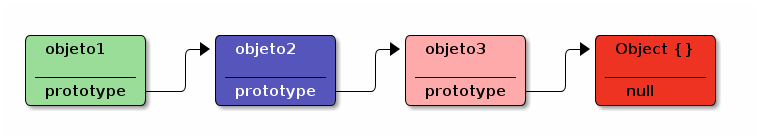
\includegraphics[width=0.7\linewidth]{imagenes/prototipo1}
\caption{Cadena prototípica de objetos}
\label{fig:cadena-prototipos}
\end{figure}

Cómo se puede observar toda cadena de prototipo acaba con el prototipo de Object, cuyo prototipo es null. Veamos algunos ejemplo de cadenas prototípicas. 

\begin{lstlisting}[language=JavaScript, numbers=left]
> var objeto = { a : 1 }; \\ cadena prototípica de objeto --> Object.prototype --> null
> Object.getPrototypeOf(o); 
  Object {}
> Object.getPrototypeOf(Object.getPrototypeOf(o));
  null

\\ cadena prototípica de una array --> Array.prototype --> Object.prototype --> null
> var array = [1,2];
> Object.getPrototypeOf(array);
  []
> Object.getPrototypeOf(Object.getPrototypeOf(array));
  Object {}
> Object.getPrototypeOf(Object.getPrototypeOf(Object.getPrototypeOf(array)));
  null
\end{lstlisting}


\subsubsection{Herencia de propiedades y métodos}

Un objeto Javascripts es un conjunto de propiedades\footnote{Los métodos son propiedades que referencia a una función} que en el momento de la herencia se copian en el nuevo objeto o objeto hijo. Así pues, en el siguiente ejemplo podemos observar como se heredan las propiedades y los "métodos". 

\begin{lstlisting}[language=JavaScript, numbers=left]
> var a = { 
	contador: 0, 
	contar : function () { 
		console.log('Contador ' + this.contador++); 
	} 
};
> a.contar();
  Contador 0
> a.contar();
  Contador 1

> var b = Object.create(a); // Crea un objeto "b" que hereda de "a"
> b.contador; // es una copia exacta de "a"
  2
> b.contar();
  Contador 2
> a.contar();  // una copia no el mismo
  Contador 2

// la cadena de prototipos de los objetos:
// b.prototype --> a.prototype --> Object.prototype --> null
\end{lstlisting}

También hay que tener especial cuidado con la palabra reservada this que siempre apunta al objeto que está heredando y no al prototipo. 

\subsubsection{Constructor, propiedad prototype y herencia}
Todos los objetos poseen un único constructor. Un constructor es sólo una función que ha sido llamada con la palabra reservada new.

Todo constructor tiene una propiedad prototype con la cual podemos definir el prototipo de todos los objetos creados con dicho constructor.

\begin{lstlisting}[language=JavaScript, numbers=left]
> var Persona = function (nombre) { 
	this.nombre = nombre;
};

> Persona.prototype = {
	saluda : function () {
		console.log('Hola soy ' + this.nombre);
	}
};

> var pepe = new Persona ("pepe");
> pepe.saluda()
  Hola soy pepe

/* prototipo de pepe --> Persona.prototype --> Object.prototype --> null */

> var juan = new Persona ("juan");
> juan.saluda()
  Hola soy juan

\end{lstlisting}

En el siguiente, ejemplo se ilustra como se puede implementar la herencia en base a un constructor y las propiedades. Para ello, vamos a basarnos en el ejemplo anterior.

\begin{lstlisting}[language=JavaScript, numbers=left]
> var Empleado = function (nombre, puesto) { 
	this.nombre = nombre;
	this.puesto = puesto;
};
> Empleado.prototype = new Persona('');
// sobreescribimos saluda
> Empleado.prototype.saluda = function () { 
	console.log('Hola soy ' + this.nombre + ' ' + this.puesto );
};

> var pepe = new Empleado ('pepe', 'programador');
> pepe.saluda();
  Hola soy pepe programador
> pepe instanceof Empleado
  true
> pepe instanceof Persona
  true
\end{lstlisting}

\subsection{Ámbito de variable (Scope)}

El ámbito de una variable\footnote{scope} es la zona del programa donde es accesible la variable. En JavaScript existen dos ámbitos: local y global.

En el ámbito global, las variables son accesibles desde cualquier punto del programa. Salvo si existe una variable con él mismo nombre en el ámbito local. 

Cuando hablamos de ámbito local, en Javascripts, nos referimos a nivel de función. Es decir, que las variables declaradas dentro de la función serán accesibles sólo dentro de la propia función. 


\begin{lstlisting}[language=JavaScript, numbers=left]
var vbleGlobal = 'Soy una variable global';

function fn (){
	var vbleLocal = "Soy una variable local";
	// vbleGlobal === 'Soy una variable global'
}

// vbleLocal === undefined 
\end{lstlisting}


\subsection{Patrón módulo}
Popularizado por Douglas Crockford el patrón módulo es sin lugar a dudas el más utilizado dentro del mundo de Javascripts. Su simplicidad encierra gran potencia y flexibilidad que han aprovechado multitud de librerías\footnote{Por citar algunas de las más populares: JQuery, Dojo y Undercore, entre otros}.  

Para definir un módulo nos basamos principalmente en dos conceptos fundamentales: 
\begin{itemize}
\item El \textbf{ámbito local}, nos va a permitir crear funciones y variables locales al módulo, es decir, privadas a nuestro módulo. 
\item Y en una \textbf{función auto-ejecutable} que retorna un objeto con el interfaz pública del módulo.
\end{itemize}

El siguiente módulo muestra un ejemplo básico de módulo\footnote{Módulo propuesto pro Douglas Crockford}.

\begin{lstlisting}[language=JavaScript, numbers=left]
// El espacio de nombres en este ejemplo es la variable "modulo"
var modulo = function () {
  // variables privadas
  var p1, p2;
 
  // funciones privadas
  function privado() {
  }
 
  // Interfaz publica
  return {
    variablePublica : null,
    funcionPublica: function () {
    }
  }
}();
\end{lstlisting}


Entre sus virtudes más destacadas están:
\begin{itemize}
\item Encapsulamiento bajo un \textbf{espacio de nombres}. Evitando colisiones de nombres con otras librerías.
\item Permite y propicia una mejor organización del código permitiendo o facilitando la \textbf{reutilización}.
\item Al quedar encapsulado bajo un espacio de nombre nos lleva a mantener un \textbf{contexto global limpio}. Sólo necesitamos de una variable global\footnote{Nos referimos al propio módulo}.
\item Concepto simple y fácilmente extensible.
\end{itemize}

En MindMapJS no es una excepción, se ha utilizado un espacio de nombres MM.\footnote{Utilizado MM (MindMap) por comodidad.} Simplemente esto:
\lstset{inputencoding=utf8/latin1}
\lstinputlisting[language=JavaScript, numbers=left]{../src/MindMapJS.js}

El módulo MM tiene el interfaz de uso para la aplicación y sobre el que gira todo comportamiento. 


\lstinputlisting[language=JavaScript, numbers=left]{../src/mm.js}

Como se puede observar se ha utilizado incorporado una pequeña variación con respecto al módulo propuesto por Douglas Crockford. Se trata de un módulo extensible. Para ello, el espacio de nombre del módulo debe estar previamente definido y posteriormente se le pasa a la función auto-ejecutable para que extienda su interfaz. Un esquema de este módulo es:

\begin{lstlisting}[language=JavaScript, numbers=left]
// El espacio de nombres en este ejemplo es la variable "modulo"
var modulo = {};

modulo = function (m) {
  // variables privadas
  var p1, p2;
 
  // funciones privadas
  function privado() {
  }
 
  m.variablePublica = null;
  
  m.funcionPublica = function () {};
 
  return m;
}(modulo);

modulo = function (m) { // extesion del modulo
  // variables privadas solo accesibles en la extension
  var p1_ext, p2_ext;
 
  // funciones privadas
  function privado_ext() {
  }
 
  m.variablePublica_ext = null;
  
  m.funcionPublica_ext = function () {};
 
  return m;
}(modulo);
\end{lstlisting}

Quedando el interfaz de nuestro módulo como la conjunción de los métodos y variables públicas definida en cada una de la extensiones.


\subsection{Implementación de MM.Class con prototipos}
Como ya hemos podido comprobar Javascripts es un lenguaje sin clases, pero podemos simular, más o menos, el comportamiento de clase. Para el proyecto he implementado un patrón de extensión que nos permite tanto heredar como implementar la sobreescritura de funciones (métodos). 


\lstinputlisting[language=JavaScript, numbers=left]{../src/klass.js}

Como se puede observar el código implementado en MM.Class.extend, se trata de una función que devuelve otra función constructora, a la cual se le ha añadido, manipulado el prototipo a partir de un objeto (prop) del que deseamos heredar o extender. Las propiedades del objeto padre, simplemente se copia pero las funciones (métodos) del objetos padre son envueltos en un closure, para poder dispones de sobreescritura de métodos. 

La función init es el constructor de nuestra clase y se llamará cuando se instancie el objeto.

\begin{lstlisting}[language=JavaScript, numbers=left]
var Persona = MM.Class.extend({
	init: function(nombre) {
		this.nombre = nombre;
	},
	bailar: function() {
		return "Si";
	},
	piernas: 2
});

var Hombre = Persona.extend({
	init: function(nombre) {
		this._super(nombre);
	},
	bailar: function() {
		return this._super() + ", pero es torpe";
	},
	
	piernas: 2,
	
	sexo: 'Hombre'
});

> var pepe = new Hombre('pepe'); // nueva instancia de hombre
> pepe.nombre;   // pepe
> pepe.bailar(); // Si, pero es torpe
> pepe instanceof Hombre; // true
\end{lstlisting}

Se puede observar en el ejemplo, como la implementación de MM.Class nos permite crear una jerarquía de clases. Además de un constructor y sobreescritura de funciones o métodos. En otras palabras, nos proporciona el mecanismo básico para sistemas más complejos. 


\subsection{Patrón Chainable.}
Popularizado por JQuery, el patrón Chainable, o encadenado, nos permite encadenar llamadas de forma que las aplicaciones pueden quedar más legibles y compactas. En MindMapJS se ha utilizado siempre que se ha podido sobre todo en el módulo MM. 

\begin{lstlisting}[language=JavaScript, numbers=left]
// ejemplo de Chainable en el MindMapJS
MM.nuevo('Como usar MindMapJS').add('Teclado').add('Raton').add('Tablet');
// Crea un nuevo mapa mental con tres nodos 
\end{lstlisting}

El patrón Chain, devuelve siempre el propio objeto del contexto de ejecución. De forma, que siempre podemos seguir realizando llamadas encadenadas. 

\lstinputlisting[language=JavaScript, numbers=left]{../src/chain.js}

En la implementación realizada se puede observar como se ha modificado el prototipo del propio objeto Function. De esta forma siempre podemos hacer nuestras funciones chain sin necesidad de acordarnos de devolver "this".

\begin{lstlisting}[language=JavaScript, numbers=left]
// ejemplo uso del patron
var mod = function (){
	return {
		saludar: function(){ console.log(" hola ") }.chain();
	};
}();
> mod.saludar().saludar().saludar() // " hola  hola  hola "
\end{lstlisting}


\subsection{Patrón publicador/suscriptor.}

Una de las grandes virtudes de NodeJS es el manejo de eventos para vertebrar distintos módulos o clases. MindMapJS también tiene un sistema de manejo de eventos. Más concretamente un patrón publicador/suscriptor. 

\lstinputlisting[language=JavaScript, numbers=left]{../src/pubsub.js}

En realidad, se trata de un patrón bastante simple, pero las posibilidades que nos proporcionan y limpieza son muy, muy importantes. Se trata de un registro de eventos y funciones callbacks a ejecutar cuando el evento publicador lo requiera. 

MindMapJS ha realizado un uso intensivo del patrón. De echo, ha permitido implementar complejos mecanismos e interacciones entre el módulo MM y el render del árbol. El siguiente código muestra como es usado en la función add crea una nueva idea en el mapa mental, y como suscrito al evento, podrá reaccionar a la creación de una nueva idea.

\begin{lstlisting}[language=JavaScript, numbers=left]
// MM eleva el evento 'add'
mm.add = function ( texto ) {
    texto = texto || 'Nueva idea';
    var nuevo = new MM.Arbol ( { id: idNodos++, texto: texto, plegado: false,  nodo: null } );
    this.foco.hijos.push ( nuevo );
    this.undoManager.add(new MM.comandos.Insertar(this.foco.elemento.id, nuevo.elemento.id, texto) );
    this.eventos.on ( 'add', this.foco, nuevo );
    nuevo = null;
}.chain();

// El render esta suscrito al evento para poder reaccionar a los 
// cambios del mapa mental.
render.prototype.suscribrirEventos = function ( ) {
    this.desuscribrirEventos(); // evitamos dobles suscripciones
    var sus = this.suscripciones;
    var e = MM.eventos;
    sus.push ( e.suscribir('ponerFoco', cambiarFoco) );
    sus.push ( e.suscribir('add', this.nuevoNodo, this) );
    sus.push ( e.suscribir('borrar', this.borrarNodo, this) );
    sus.push ( e.suscribir('nuevo/pre', function () {
        MM.arbol.elemento.nodo.destroy();
    }) );
    sus.push ( e.suscribir('nuevo/post', function () {
        this.renderizar();
    }, this) );
    this.contenedor.addEventListener("mousewheel", handlerWheel, false);
    this.contenedor.addEventListener("DOMMouseScroll", handlerWheel, false);
    sus = e = null;
};
\end{lstlisting}

Las funciones callbacks asociadas a un evento se apilan y se ejecutan en orden de registro. Así pues, puede existir distintos puntos dentro de la aplicación donde tratar el evento.

\subsection{UndoManager.}
El comportamiento de esta clase ya fue explicado con su diagrama de clase y en la figura\ref{fig:undomanager-ejecucion} en este apartado vamos a destripara un poco más su comportamiento.

\begin{figure}[tbph]
\centering
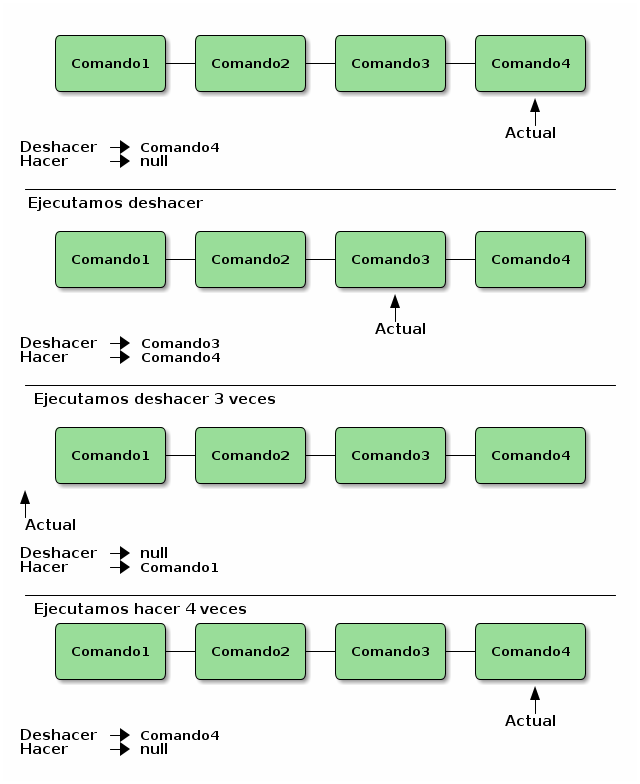
\includegraphics[width=0.7\linewidth]{imagenes/undomangerEjecucion.png}
\caption{Secuencia de ejecución de UndoManager}
\label{fig:undomanager-ejecucion}
\end{figure}

La idea primigenia es posibilitar al usuario final de la aplicación la opción de deshacer y rehacer las acciones ejecutadas en el MindMapJS. UndoManager mantiene en un array los comandos realizados y un puntero (actual) que apunta a la última comando realizado. También disponemos de un limite de comandos(maxComandos) apilados en el historial. 

El interfaz de la clase MM.UndoManager nos permite añadir nuevos comandos al historial, hacer y deshacer, conocer el estado del historial y el nombre del siguiente comando hacer o deshacer. También se le ha incorporado un manejador de eventos para que, los usuarios de la clase puedan saber en todo momento los cambios sufridos en el historial.

\lstinputlisting[language=JavaScript, numbers=left]{../src/undoManager.js}

La clase base de todos los comandos hacer y deshacer es MM.UndoMangaer.ComandoHacerDeshacer. Esta clase implementa un patrón comando con una variante obvia, que en realidad tiene registra dos comandos. Uno para hacer y otro para deshacer. 

\lstinputlisting[language=JavaScript, numbers=left]{../src/undoManager.js}

\section{Concatenación y UglifyJS}
Es conveniente la unificación y compresión de código Javascripts. Con ello, no sólo reducimos el número de peticiones\footnote{Más concretamente peticiones http get}, desde el navegador al servidor, sino que optimizamos los tiempos de carga y respuesta del navegador. Este aspecto es siempre deseable, evitando al usuario final esperas indeseadas.  

Se ha utilizado la herramienta UglifyJS\footnote{En combinación con GruntJS} en MindMapJS, no sólo por tratarse de una librería estándar dentro de herramientas de ofuscación y reducción de código Javascript, sino por los beneficios que nos aporta.

Es sencillo, comprobar que se reduce considerablemente el tiempo, si se concatenan los ficheros Javascript. Por cada fichero Javascript el navegador realiza una petición Get como se puede comprobar en la imagen \ref{fig:carga-desarrollo}.  

\begin{figure}[tbph]
\centering
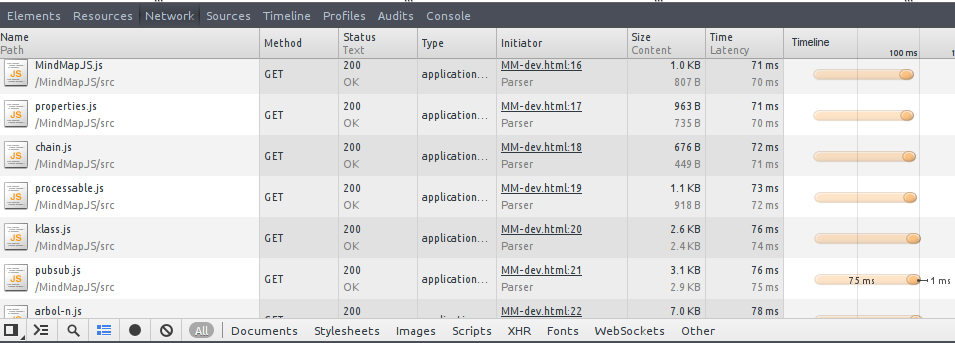
\includegraphics[width=0.9\linewidth]{imagenes/Uglify1.png}
\caption{Carga de ficheros Javascript en desarrollo}
\label{fig:carga-desarrollo}
\end{figure}

Cada solicitud de fichero, por parte del navegador, tiene una latencia de red y un tiempo de carga por parte de navegador que puede provocar, dependiendo de las condiciones y velocidad de la red utilizada, esperas en por parte de usuario final. En la siguiente captura \ref{fig:carga-concatenado}, veremos como al concatenar reducimos el número de peticiones realizadas al servidor y por lo tanto, el tiempo de carga\footnote{Más concretamente a sólo 16ms en un fichero un único fichero de 111Kb.}.

\begin{figure}[tbph]
\centering
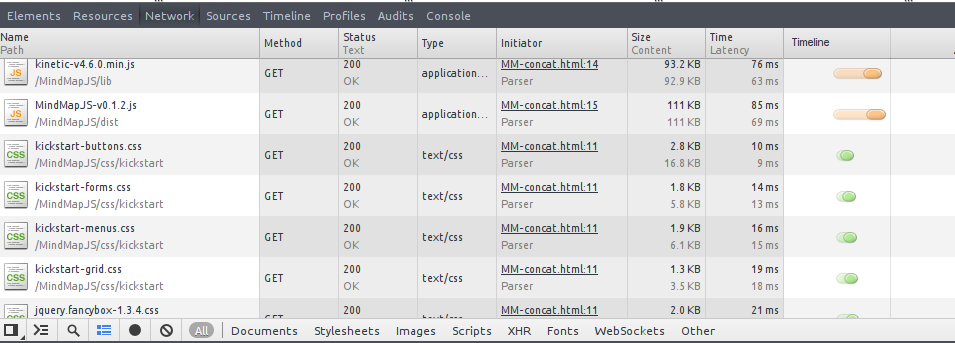
\includegraphics[width=0.9\linewidth]{imagenes/Uglify2.png}
\caption{Carga de ficheros Javascript concatenado}
\label{fig:carga-concatenado}
\end{figure}

Si a su vez comprimimos y reducimos al máximo el tamaño del fichero con UglifyJS, podemos comprobar, en la figura \ref{fig:carga-comprimido}, como el tiempo de carga de la librería se reduce considerablemente. 

\begin{figure}[tbph]
\centering
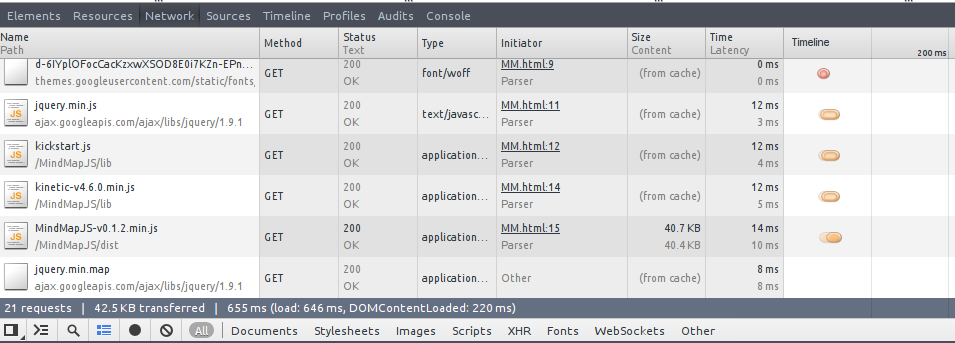
\includegraphics[width=0.9\linewidth]{imagenes/Uglify3.png}
\caption{Carga de ficheros Javascript comprimido}
\label{fig:carga-comprimido}
\end{figure}

Más concretamente, podemos comprobar que el fichero se a reducido desde los 111 Kbytes a 40.7 Kbytes. Es decir, se ha reducido el tamaño del fichero más de 35\% y el tiempo de carga a tan sólo 4 ms. 

Como se puede comprobar es deseable la concatenación y reducción del código en toda aplicación web. Ya que el tiempo de respuesta y la experiencia de usuario mejoran al evitar tiempos muertos en la carga. Sobre todo en sistemas donde el ancho de banda es reducido. 


\section{JsHint}
JsHint es otra herramienta que no debe faltar en ningún desarrollo web. En MindMapJS se ha utilizado continuamente en los periodos de desarrollo. JsHint nos permite comprobar la validez y calidad de nuestro código Javascript, analizando del código fuente y mostrándonos los puntos en los que puede mejorarse desde el punto de vista de las buenas prácticas y código limpio. Evitando pues, errores o posibles errores de interpretación del código fuente.

He utilizado JsHint por que se trata de un estándar utilizado por multitud de desarrollares web y que tiene una gran aceptación por parte de los grandes la programación web. Salvo quizás Douglas Crockford, autor de la herramienta JSLint.

JSLint es un validador de código muy exhaustivo y da muchos falsos positivos. Además tiene muchos detractores, que alegan que los criterios evaluados son bastante subjetivos, sigue los criterios impuestos por Douglas Crockford\footnote{su creador}. Por todo ello, algunos desarrolladores crearon un fork llamado JSHint con el objeto de mejorar las mediciones que eran bastante arbitrarias en JSLint.

\section{KineticJS}
KineticJS es un framework gráfico sobre el canvas de HTML5, permitiendo anidamiento de nodos, capas, filtros, animaciones y manejo de eventos de forma muy sencilla. 

La librería KineticJS tiene en lo alto de la jerarquía de Objetos al escenario que puede tener una o más capas. Cada capa se renderiza en dos canvas, uno para contener los elementos gráficos y otro oculto para agilizar y aclarar la detección de eventos. Cada capa puede contener cualquier elemento gráfico.

\begin{figure}[tbph]
\centering
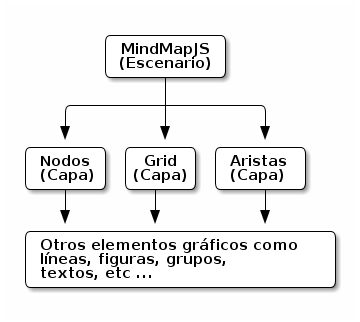
\includegraphics[width=0.6\linewidth]{imagenes/diagrama-kineticjs.png}
\caption{Escenario y modelo de capas KineticJS de MindMapJS}
\label{fig:escenario-capas}
\end{figure}


\subsection{¿Por qué usar KineticJS?}
Entre otras virtudes, lo que más me atrajo a la hora de utilizar KineticJS es:
\begin{itemize}
\item \textbf{Su rendimiento.} Presenta un muy buen rendimiento gráfico. 
\item \textbf{Soporte para capas.} Manejo sencillo de capas permitiendo sobreponer capas.
\item \textbf{API clara y extensible.} Presenta un código claro, orientado a objetos y eventos. Resulta sumamente sencillo extender la librería como se puede ver en el apartado 'Extendiendo KineticJS'.
\item \textbf{Manejo de eventos.} No sólo a nivel de canvas. También a nivel de figura. Soporta multitud de eventos no sólo de escritorio sino también de dispositivos táctiles.
\item \textbf{Continuo desarrollo.} El desarrollo y avance de la librería es notable y tiene una comunidad detrás proporcionando ideas, soluciones, y verificando el desarrollo del la librería.
\end{itemize}

\subsection{Algunos ejemplos sencillos.}
Para todos los ejemplos sobre KineticJS a partir de ahora vamos a utilizar el mismo modelo de página HTML5. En ella, incorporaremos la librería de KineticJS y un contenedor para nuestro lienzo. Una etiqueta div que posteriormente utilizaremos para indicarle a KineticJS donde tiene que pintar.
 
\lstinputlisting[language=HTML, numbers=left]{../test/kineticJS/1_eventos.html}

\subsection{Creando escenarios y capas.}

En este ejemplo vamos a crear un escenario y le incorporaremos una capa donde se dibujará un texto. En la figura \ref{fig:kinetic-ejemplo-escenarios-capas} podemos comprobar el resultado final.

\begin{figure}[tbph]
\centering
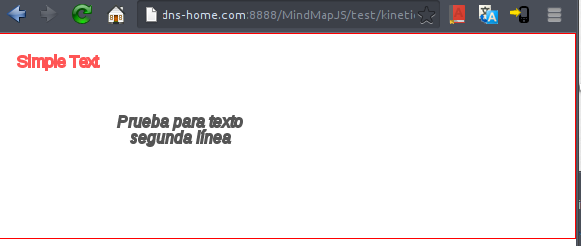
\includegraphics[width=0.6\linewidth]{imagenes/KineticjsEjemplo0.png}
\caption{Ejemplo de Kinetic - uso básico de capas}
\label{fig:kinetic-ejemplo-escenarios-capas}
\end{figure}

\lstinputlisting[language=JavaScript, numbers=left]{../test/kineticJS/0_texto.js}

El ejemplo muestra en la línea 34 como se crea un escenario (Kinetic.Stage) indicando el contenedor dentro nuestro árbol DOM y su dimensiones. A continuación (en la línea 40) creamos una capa (Kintetic.Layer) donde dibujaremos los elementos gráficos que deseamos pintar. Más concretamente se ha creado dos elementos Kinetic.Text y se han incorporado a la capa.

Se trata de un concepto muy utilizado en editores gráficos, por nombrar algunos, como Gimp y PhotoShop. Es exactamente el mismo concepto. En MindMapJS se ha utilizado concretamente tres capas superpuestas en el siguiente orden:
\begin{itemize}
\item \textbf{Capa grid:} muestra la rejilla de fondo.
\item \textbf{Capa aristas:} contiene todas las aristas que interconecta las ideas. 
\item \textbf{Capa nodos:} contiene las ideas que representan el mapa mental.
\end{itemize}


\subsection{Manejo de eventos.}
Como se ha expresado con anterioridad tiene un buen sistema para manejo de eventos tanto de escritorio como touch. En el siguiente ejemplo \ref{fig:kinetic-ejemplo-eventos} podemos ver como manejar eventos sobre objetos con KineticJS.

\begin{figure}[tbph]
\centering
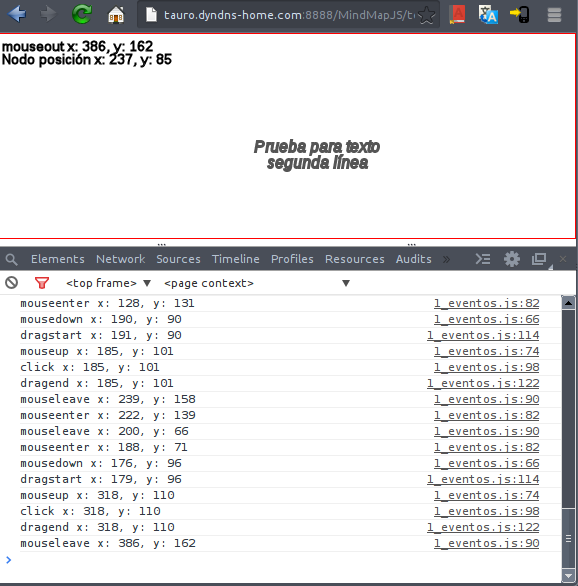
\includegraphics[width=0.6\linewidth]{imagenes/KineticjsEjemplo1.png}
\caption{Ejemplo de Kinetic - eventos}
\label{fig:kinetic-ejemplo-eventos}
\end{figure}

\lstinputlisting[language=JavaScript, numbers=left]{../test/kineticJS/1_eventos.js}

Podemos ver que sigue un modelo de eventos estilo JQuery en el cual nos suscribimos a un evento mediante la fórmula: \footnote{También implementada en MindMapJS} 
\begin{lstlisting}[language=JavaScript, numbers=left]
ElementoGrafico.on('nombreEvento', function () { 
	// Manejo del evento.
});
\end{lstlisting}

Con este modelo, cualquier programador Javascript familiarizado con JQuery entiende como se comporta y sabe de inmediato como utilizarlo.  

Existen otro muchos ejemplos que podemos ver y manipular en la página tutorial de KineticJS\footnote{Tutoriales en http://www.html5canvastutorials.com/kineticjs/html5-canvas-kineticjs-shape-tutorial/}. 

\subsection{Extendiendo KineticJS.}

Existen dos formas de crear y extender KineticJS. La primera es mediante la creación de 'custom shape', se trata de un mecanismo para poder crear figuras que nosotros deseemos pintando directamente en el canvas. La segunda es implementación de una clase y extender su comportamiento dotando a nuestro nuevo elemento gráfico todas la virtudes de cualquier figura KineticJS.

\begin{figure}[tbph]
\centering

\includegraphics[width=0.6\linewidth]{imagenes/KineticjsEjemplo2.png}
\caption{Ejemplo de Kinetic - custom shape}
\label{fig:kinetic-ejemplo-customshape}
\end{figure}

La creación de 'custom shape' se basa en la implementación de una función (sceneFunc) que será utilizada a la hora de dibujar la figura. Esta función recibe un canvas sobre el que podemos dibujar directamente. 

\begin{lstlisting}[language=JavaScript, numbers=left]
	var stage = new Kinetic.Stage({
        container: 'container',
        width: 578,
        height: 200
    });
    var layer = new Kinetic.Layer();

    var triangle = new Kinetic.Shape({
        sceneFunc: function(context) {
          context.beginPath();
          context.moveTo(200, 50);
          context.lineTo(420, 80);
          context.quadraticCurveTo(300, 100, 260, 170);
          context.closePath();
          context.fillStrokeShape(this);
        },
        fill: '#00D2FF',
        stroke: 'black',
        strokeWidth: 4
    });

    layer.add(triangle);
    stage.add(layer);
\end{lstlisting}

Esta segunda forma de extensión tiene la ventaja de que nos permite crear una clase que podremos reutilizar cada vez que necesitemos. Este mecanismo ha sido el utilizado para crear las aristas de MindMapJS implementando, como podemos comprobar en el siguiente código, una curva beizer para estos propósitos. Se trata, en definitiva, de crear una nueva función constructora y definir su prototipo en el cual no puede faltar la función init y drawFunc. 

\lstinputlisting[language=JavaScript, numbers=left]{../src/beizer.js}


\section{NodeJS}

Basado en la máquina virtual Javascripts V8 de Google, NodeJS\footnote{La web oficial de NodeJS es nodejs.org} a supuesto una revolución en el mundo de la programación Javascripts, dando un salto de gigante desde el lado del cliente al servidor. Este enorme evolución, y de manos de V8, ha provocado la creación de un entorno de programación completo, en el cual se aglutina desde un REPL\footnote{Patrón Read-Eval-Print Loop} para pruebas y depuración interactiva hasta un gestor de paquetes y librerías NPM\footnote{La web oficial de NPM es npmjs.org} (Node Packaged Modules).

\begin{wrapfigure}{l}{0.4\textwidth}
  \begin{center}
    
\includegraphics[width=0.2\textwidth]{imagenes/nodejs-light}
  \end{center}
  \caption{Logo NodeJS}
  \label{fig:nodejs}
\end{wrapfigure}

NodeJS nos permite crear aplicaciones de red escalables, alcanzando un alto rendimiento utilizando entrada/salida no bloqueante y un bucle de eventos en una sola hebra. Es decir, que NodeJS se programa sobre un sólo hijo de ejecución y en el caso de que necesite operaciones de entrada/salida, creará una segunda hebra para evitar su bloqueo. En teoría NodeJS puede mantener tantas conexiones simultaneas abiertas como descriptores de fichero soporte el sistema operativo (en UNIX aproximadamente 65.000), en la realidad son bastantes menos (se calcula que entre 20.000 y 25.000). 

Como ya se ha mencionado, y debido a que su arquitectura es usar un único hilo, sólo puede unas una CPU. Es el principal inconveniente que presenta la arquitectura de NodeJS.

Sus principales objetivos son:
\begin{itemize}
\item Escribir aplicaciones eficientes en entrada y salida con un lenguaje dinámico.
\item Soporte a miles de conexiones.
\item Evitar las complicaciones de la programación paralela (Concurrencia vs paralelismo).
\item Aplicaciones basadas en eventos y callbacks.
\end{itemize}

\subsection{Instalación de NodeJS}
Existen varias formas de instalar NodeJS, por ejemplo, utilizando los repositorios del sistema operativo o instaladores. En mi caso, he utilizado la compilación del código fuente que esta alojado en GitHub\footnote{Repositorio de NodeJS https://github.com/joyent/node}. 

Lo primero que tenemos debemos hacer es clonar el proyecto.

\begin{lstlisting}[language=bash, numbers=none]
$ git clone git://github.com/joyent/node.git
$ cd node
\end{lstlisting}

Una vez tengamos la copia del código fuente realizaremos un checkout de una versión estable.

\begin{lstlisting}[language=bash, numbers=none]
$ git branch vXXXX Nombre
$ git checkout Nombre
\end{lstlisting}

Ahora, ya estamos en disposición de compilar el fuente de la versión estable. 

\begin{lstlisting}[language=bash, numbers=none]
$ ./configure --prefix=/usr/local 
$ sudo make install
\end{lstlisting}

\subsection{Instalación del NPM}
Como ya se ha comentado antes NPM\footnote{Node Packaged Module (NPM) web oficial npmjs.org} es el gestor de paquetes de NodeJS. En la versiones actuales ya viene instalado, pero eso no fue siempre así. También se puede optar por instalarse de sin
NodeJS. Para ello, ejecutaremos el siguiente comando:

\begin{lstlisting}[language=bash, numbers=none]
$ curl https://npmjs.org/install.sh | sh
\end{lstlisting}

\subsection{Uso básico de NPM}

\subsubsection{Iniciar un proyecto nuevo}

A continuación se muestra la secuencia de comandos necesaria para crear un proyecto.

\begin{lstlisting}[language=bash, numbers=none]
$ mkdir hola
$ cd hola
$ npm init
npm init
This utility will walk you through creating a package.json file.
It only covers the most common items, and tries to guess sane defaults.

See `npm help json` for definitive documentation on these fields
and exactly what they do.

Use `npm install <pkg> --save` afterwards to install a package and
save it as a dependency in the package.json file.

Press ^C at any time to quit.
name: (hola) 
version: (0.0.0) 
git repository: 
author: 
license: (BSD-2-Clause) 
About to write to /tmp/hola/package.json:

{
  "name": "hola",
  "version": "0.0.0",
  "description": "Hola mundo",
  "main": "index.js",
  "scripts": {
    "test": "echo \"Error: no test specified\" && exit 1"
  },
  "keywords": [
    "hola",
    "mundo"
  ],
  "author": "",
  "license": "BSD-2-Clause"
}

Is this ok? (yes) 
\end{lstlisting}

El comando \textbf{npm init} comenzará a realizarnos preguntas sobre los datos del proyecto como nombre, versión, etc. Una vez terminado, tendremos nuestro fichero de configuración (package.json) preparado.

\subsubsection{Buscar paquetes y obtener información}

El primer comando nos permite buscar paquetes interesantes o útiles a nuestro proyecto, y el segundo, para obtener una descripción más exhaustiva del mismo.

\begin{lstlisting}[language=bash, numbers=none]
$ npm search <palabra>:
$ npm info <paquete>
\end{lstlisting}

\subsubsection{Instalación de paquetes}

Existen varias formas para instalar un paquete y/o librería. 

De forma global \footnote{Con el modificador -g} para que lo puedan utilizar todas las librerías del sistema.

\begin{lstlisting}[language=bash, numbers=none]
$ npm install <paquete> -g
\end{lstlisting}

De forma local\footnote{Sin el modificador -g}, es decir, sólo se podrá utilizar el proyecto actual.

\begin{lstlisting}[language=bash, numbers=none]
$ npm install <package name>
\end{lstlisting}

También existen dos modificadores muy interesantes \textit{--save} para que se incluya (en el fichero package.json) la librería o paquete como dependencia del proyecto. Y el otro modificador es \textit{--save-dev} para que la dependencia sea de desarrollo. Así quedaría un fichero package.json después de haber incluido un paquete (colors) como dependencia y otro (grunt-cli) como dependencia de desarrollo.

\begin{lstlisting}[language=JavaScript, numbers=left]
{
  "name": "hola",
  "version": "0.0.0",
  "description": "Hola mundo",
  "main": "index.js",
  "scripts": {
    "test": "echo \"Error: no test specified\" && exit 1"
  },
  "keywords": [
    "hola",
    "mundo"
  ],
  "author": "",
  "license": "BSD-2-Clause",
  "dependencies": {
    "colors": "~0.6.2"
  },
  "devDependencies": {
    "grunt-cli": "~0.1.9"
  }
}
\end{lstlisting}

\subsubsection{Desinstalación de paquetes}

Las instrucciones son la misma salvo por que el comando \textit{install} se sustituye por \textit{uninstall}.

\subsection{¿Por qué utilizar NodeJS y NPM?}
Sin lugar a dudas se trata de herramientas potentes que proporcionan al desarrollador un buen punto de partida para cualquier desarrollo Javascripts. Lo que me decidió por NodeJS, desde un principio, fue:

\begin{itemize}
\item Disponer de una \textbf{consola} que me permita probar algunas partes del desarrollo sin necesidad de un navegador. Agilizando así el desarrollo de algunas librerías.
\item Tener disponible un \textbf{sistema de paquetes como NPM} que me permite integrar multitud de librerías para el desarrollo, de forma sencilla y eficaz. 
\item La amplia aceptación de esta herramienta y la multitud de \textbf{librerías} implementadas para la plataforma. Entre ellas, están todas la herramientas utilizadas en MindMapJS. Librerías para gestión de tareas\footnote{GruntJS ha sido la elección utilizada como gestor de tareas}, pruebas\footnote{En el caso de las pruebas unitarias opté por MochaJS} y verificación de código\footnote{JsHint} entre otras muchas. 
\end{itemize}
\section{GruntJs}

Se trata de una aplicación Node que está empaquetada y disponible en NPM. GruntJS es una herramienta versátil para la automatización de tareas mediante Javascripts, evitándonos dentro de lo posible la realización de tareas repetitivas. Con un simple archivo de configuración nos permite realizar tareas tan diversas como minificar código, lanzar la suite de tests, etc.


\subsection{Características}

\begin{itemize}
\item \textbf{Acceso a archivos:}
	No tenemos que preocuparnos del acceso a archivos, sólo tratarlos.	
\item \textbf{Automatización de tareas y conjunto de tareas:}
	Podemos automatizar pequeñas tareas o mediante un conjunto de ellas automatizar tareas más complejas como la comprensión de una librería Javascripts. 
\item \textbf{Fácil instalación:}
	Esta en NPM, la instalación es simplemente un npm install.
\item \textbf{Plugins comunitarios:}
	Existe un gran comunidad detrás creando plugins, que podemos utilizar utilizando NPM.
\item \textbf{Multi-plataforma:}
	Al ser una librería Node nos permite utilizarlo en cualquier plataforma que soporte Node.
\end{itemize}

\subsection{Instalación}
La instalación de GruntJS no tiene complicación, ya que, al tratarse de una aplicación Node y estar publicado en NPM sólo necesitamos como prerrequisito tener instalado Node y NPM.

Lo primero es instalar el cliente de forma global con el comando:

\begin{lstlisting}[language=bash, numbers=none]
$ npm install grunt-cli -g
\end{lstlisting}

\begin{wrapfigure}{r}{0.4\textwidth}
  \begin{center}
    
\includegraphics[width=0.2\textwidth]{imagenes/grunt-logo}
  \end{center}
  \caption{Logo GruntJS}
  \label{fig:gruntjs}
\end{wrapfigure}

Y una vez instalado el cliente, en nuestro proyecto debemos ejecutar:

\begin{lstlisting}[language=bash, numbers=none]
$ npm install grunt --save-dev
\end{lstlisting}

Ya tenemos agregado GruntJS a nuestro proyecto. Con los --save-dev le indicamos al NPM que lo añada a las dependencias del proyecto para desarrollo. Así incluirá las líneas pertinentes en nuestro fichero package.json.

\begin{lstlisting}[language=JavaScript, numbers=left]
{
  "name": "nombre",
  "version": "0.0.1",
  "dependencies": { 
 
  },
  "devDependencies": {
    "grunt": "~0.4.1"
  }
}
\end{lstlisting}


\subsection{Creando el Gruntfile}
En el fichero Gruntfile.js será donde definamos las tareas que deseamos en nuestro proyecto. El esquema de fichero es:

\begin{lstlisting}[language=JavaScript, numbers=left]
module.exports = function(grunt) {
 
  grunt.registerTask('default', 'Tarea Hola Mundo', function() {
    grunt.log.write('Hola Mundo!').ok();
  });
 
};
\end{lstlisting}

Como se puede observar se trata de un modulo Node, que será llamado por grunt cuando lo ejecutemos. En el ejemplo, le hemos registrado una tarea por defecto que imprime "Hola Mundo!". Ahora sólo tenemos que ejecutar el comando grunt para ver el resultado de nuestra tarea.

GruntJS tiene un conjunto básico de plugins, nombrados grunt-contrib-XXXX, empaquetados en NPM y que podemos instalar fácilmente. 

\subsection{Gruntfile.js de MindMapJS}

El fichero de configuración de GruntJS utilizado para el proyecto es :

\lstinputlisting{recursos/Gruntfile.js}

Como se puede comprobar se han incorporados distintos plugins:

\begin{itemize}
\item \textbf{grunt-contrib-concat:} permite concatenar un conjunto de ficheros en nuestro caso los ficheros Javascripts.
\item \textbf{grunt-replace:} plugins para realizar operaciones de reemplazo dentro de un conjunto de ficheros.
\item \textbf{grunt-contrib-uglify:} para comprimir y/o minimizar el código Javascripts.
\item \textbf{grunt-contrib-clean:} borrar un conjunto de ficheros o el contenido de un directorio.
\item \textbf{grunt-contrib-jshint:} permite realizar la verificación y validación de buenas prácticas establecidas en Javascripts.
\item \textbf{grunt-jsdoc:} compilar los comentarios JSDocs para generarla documentación HTML del API.
\item \textbf{grunt-mocha-test:} tarea que lanza la suite de tests unitarios del proyecto.
\end{itemize}

Con estos plugins se han cubierto todas las necesidades de automatización de tareas del proyecto. Las tareas implementadas son:

\begin{itemize}
\item \textbf{dev:} que concatena el código fuente y realiza los reemplazo como fechas, versión, etc ...
\item \textbf{full:} además de realizar las tareas propias de la tarea 'dev', minimiza y realiza los reemplazos de producción.
\item \textbf{test:} lanza la suite de test
\item \textbf{hint:} lanza la tarea de validación de código JSHint.
\item \textbf{jsdoc:} genera la documentación del API.
\end{itemize}

\subsection{¿Por qué GruntJs?}
En cualquier desarrollo surgen multitud de tareas repetitivas que pueden llegar a ralentizar la elaboración de cualquier aplicación. 

GruntJs está empaquetado en el sistema NPM, por lo que, es se puede instalar con un sencillo comando NPM. Pero su fuerza radica en que, se programan las tareas en Javascripts de forma sencilla y clara. Permitiendo al programador la posibilidad de extenderlo mediante un sistema de plugins. 

Esta siendo ampliamente utilizado por JQuery, Modernizr, Bootstrap y WordPress Build Process. Por nombrar algunos de los más destacados.  

\section{Github}


Todo proyecto que se precie debe estar sustentado con sistema de control de versiones, en nuestro caso ha sido Git\footnote{Web oficial de Git es git-scm.com}. Más concretamente se trata de un sistema distribuido de control de código fuente o SCM\footnote{SCM (Source Code Management)} creado por Linus Torvalds, a partir, de su propia experiencia en el desarrollo de los kernels de Linux. 

Github\footnote{La web de Github es github.com} es una plataforma online pensada para el desarrollo colaborativo de proyectos, utilizando para ello Git. Github nos permite almacenar de forma pública\footnote{Github permite crear proyectos privados con cuentas de pago} nuestro código fuente, promoviendo el trabajo colaborativo entre profesionales. Así pues, otro profesional ajeno al proyecto puede solicitar cambios sugerir mejoras o reportar bugs.

\begin{wrapfigure}{l}{0.4\textwidth}
  \begin{center}
    
\includegraphics[width=0.48\textwidth]{imagenes/octocat}
  \end{center}
  \caption{Mascota de Github}
	\label{fig:octocat}
\end{wrapfigure}

De las características mas resaltables de Github para el control de versiones, podemos enumerar las siguientes:
\begin{itemize}
\item \textbf{Wiki para el proyecto}, con el principal propósito de documentar nuestro proyecto Github nos proporciona una Wiki. 
\item \textbf{Gráficas}, tiene un conjunto de gráficas detalladas para determinar el avance del proyecto y el progreso de cada colaborador del proyecto.
\item \textbf{Página web del proyecto}, para presentar nuestro proyecto y/o repositorio 
\end{itemize}

Como sistemas de colaboración entre programadores tenemos el:
\begin{itemize}
\item \textbf{Fork}, con un fork podemos clonar un repositorio para realizar cambios que necesitemos, de forma que podamos adaptar el proyecto a nuestras necesidades concretas. Un fork nos permite colaborar con el proyecto original mediantes los pull requests.
\item \textbf{Pull requests}, una vez realizados los cambios, y si lo vemos oportuno, podemos reportar las variaciones al proyecto original mediante un pull request. El pull request pueden ser cambios, mejoras en la funcionalidad, y/o correcciones, que deberá aprobar él/los programadores del proyecto original. 
\end{itemize}

\subsection{Crear el repositorio}
Previo a la creación del repositorio debemos crearnos una cuenta de usuario en Github. una vez realizado, sólo debemos pulsar la opción de "new repository". Ahora, ya tenemos repositorio pero debemos dotarlo de contenido, y para ello, y desde una consola local realizaremos:

\begin{itemize}
\item Creamos el directorio del proyecto.
\begin{lstlisting}[language=bash, numbers=none]
$ mkdir ~/proyecto
$ cd proyecto
\end{lstlisting}

\item Iniciamos el repositorio git
\begin{lstlisting}[language=bash, numbers=none]
$ git init
\end{lstlisting}

\item Creamos el fichero README.md. Se trata de un fichero con formato markdown\footnote{http://es.wikipedia.org/wiki/Markdown} en el cual hay que introducir un descripción del proyecto. Este fichero se visualizará en le página principal del repositorio. 

\item Añadimos y confirmamos los cambios.
\begin{lstlisting}[language=bash, numbers=none]
$ git add .
$ git commit -m 'primer commit'
\end{lstlisting}

\item Cambiamos el remote origin a la ruta de nuestro repositorio.
\begin{lstlisting}[language=bash, numbers=none]
$ git remote add origin https://github.com/usuario/proyecto.git
\end{lstlisting}

\item subimos los cambios al repositorio
\begin{lstlisting}[language=bash, numbers=none]
$ git push origin master
\end{lstlisting}

\end{itemize}

\subsection{Fork/Pull request}

Crear un fork de un proyecto utilizando Github es trivial. Tan sólo hay que ir al proyecto en cuestión y pulsar el botón de fork. Github crea una copia del proyecto de forma que si el proyecto original tiene la url https://github.com/usuariOriginal/proyecto.git y la copia tendrá la url https://github.com/usuario/proyecto.git. Ahora ya estamos en disposición de trabajar clonando el repositorio:

\begin{lstlisting}[language=bash, numbers=none]
$ git clone https://github.com/usuario/proyecto.git
\end{lstlisting}

Ya tenemos el repositorio listo para su uso. Si deseamos colaborar con el proyecto original debemos crear una rama\footnote{Operaciones a realizar: branch y checkout}, realizar los cambios y subirlos\footnote{Operaciones a realizar: commit y push} a nuestro fork de Github.  Desde Github procede realizar la revisión de los cambios y pulsar sobre la opción de 'create a pull request for this comparison'.


\section{JSDoc}

Tan importante como el código es la documentación del mismo, JSDoc\footnote{Url del proyecto https://github.com/jsdoc3/jsdoc} es una herramienta inspirada en Javadoc\footnote{http://es.wikipedia.org/wiki/Javadoc} pero pensada para Javascript. 

Mediante una conjunto de etiquetas (@class, @function, etc) introducidas como comentarios del código fuente,  se generará la documentación en formato HTML\footnote{Por lo general, se genera HTML pero permite otros formatos como RTF.}. Todos los desarrolladores que alguna vez hemos programado en Java y generado documentación de nuestro código, en JavaDoc, estamos familiarizados con el mecanismo de etiquetas, por lo que resulta muy intuitivo la elaboración de la documentación. 

En la figura \ref{fig:codigoconjsdoc} se puede ver un ejemplo de uso de las etiquetas en el código fuente. En concreto de una clase PubSub del propio proyecto MindMapJS. Se puede observar claramente, como se usan etiquetas como @author, @versión, @constrcutor, @class, etc ...  

\begin{figure}[htbp]
\centering
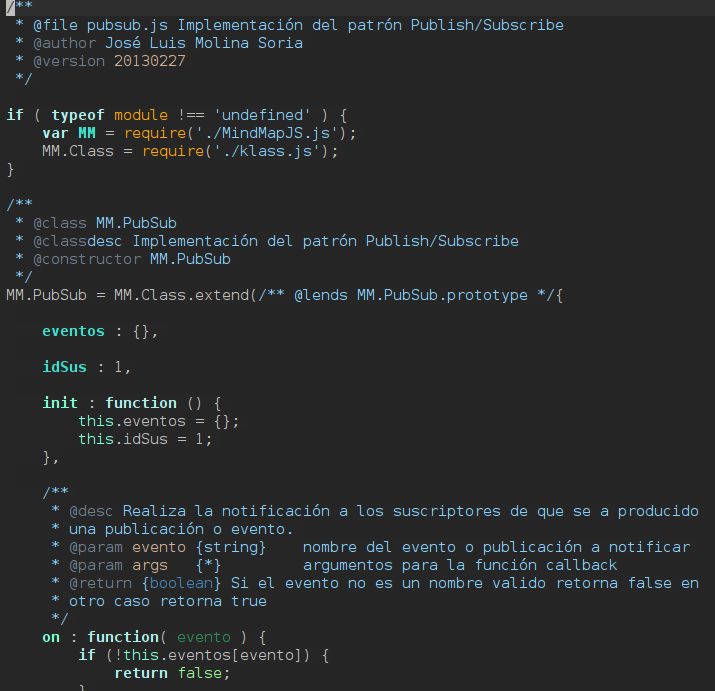
\includegraphics[width=0.7\textwidth]{imagenes/codigoconjsdoc}
\caption{Ejemplo de código fuente documentado con JSDoc}
\label{fig:codigoconjsdoc}
\end{figure}


En la figura \ref{fig:jsdoc} tenemos el resultado de compilar el código fuente con JSDoc. El resultado es un HTML que podemos retocar y configurar, permitiendo tener una Wiki, vistosa y funcional, de la documentación de nuestro cógido fuente.

\begin{figure}[htbp]
\centering
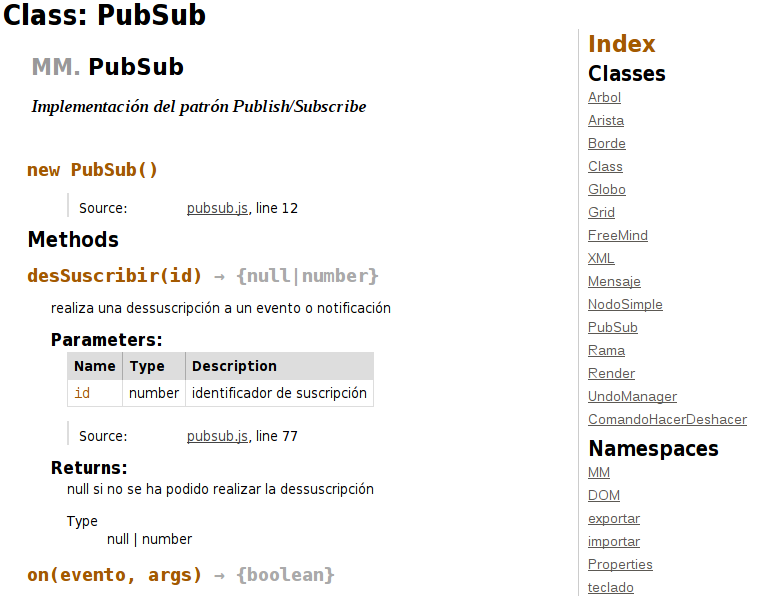
\includegraphics[width=0.7\textwidth]{imagenes/jsdoc}
\caption{Página generada por JSDoc}
\label{fig:jsdoc}
\end{figure}


\section{Mocha}

Mocha\footnote{Página oficial de Mocha: http://visionmedia.github.io/mocha/} es un framework Javascripts para realizar pruebas unitarias. Sus creadores lo definen como:

\begin{quote}
\textit{Mocha is a feature-rich JavaScript test framework running on node.js and the browser, making asynchronous testing simple and fun. Mocha tests run serially, allowing for flexible and accurate reporting, while mapping uncaught exceptions to the correct test cases. Hosted on GitHub.}
\end{quote}


Y sinceramente, creo que la definición no puede ser más acertada. Permite crear test con relativa facilidad y con una sintaxis clara y concisa. De puedo decir, que es ''simple, flexible y divertido''\footnote{En la cabecera de su web podemos leer "mocha simple, flexible, fun"}.


\subsection{Características}

Entre sus características más destacables están:


\begin{itemize}
\item \textbf{Soporte para NodeJs.} No sólo soporta el uso con NodeJS sino que esta empaquetado para NPM, por lo que, la instalación y la puesta en marcha resulta muy, muy sencilla. También existen plugins para utilizarlo con GruntJs.
\item \textbf{Soporte para diferentes navegadores.} Por lo que, podemos probar nuestro interfaz en el navegador y verificar su correcto funcionamiento.
\item \textbf{Informes.} Tiene opciones para generar informes en varios formatos dependiendo de las necesidades.
\item \textbf{Uso de cualquier librería de afirmaciones(Assertions).} Existe principalmente cuatro librerías que pueden ser utilizadas con Mocha Chai, Should, Expect y Better-Assert.
\item \textbf{Soporte para test síncronos y asíncronos.} Permite abarcar todas las necesidades de nuestro código.
\end{itemize}

\subsection{Ejemplo}

\begin{wrapfigure}{r}{0.2\textwidth}
  \begin{center}
    \includegraphics[width=0.2\textwidth]{imagenes/mocha-logo}
  \end{center}
  \caption{Mocha}
	\label{fig:mocha}
\end{wrapfigure}


He aquí un simple ejemplo de uso de mocha. 

\lstinputlisting{recursos/array-test.js}


Para empezar, debe realizar importar la librería de afirmaciones (assertions) que vamos a utilizar en el presente ejemplo se ha utilizado assert\footnote{En MindMapJS se ha utilizado Should y Chai}. 

Las líneas 2 y 3 describen a su vez, un módulo y submódulo de ejecución. En nuestro caso el módulo lo hemos llamado "Array" y el submódulo de ejecución "indexOf()". Conviene ser descriptivos en los nombres de los módulos y submódulos. 

La línea 4 describe una prueba unitaria a la que le asociamos una función anónima con las afirmaciones necesaria.

Una vez escrita la prueba unitaria ejecutamos el siguiente comando “mocha -R *.js” obtenemos el resultado que podemos observar en la figura \ref{fig:mochaejecucion}.

\begin{figure}[htbp]
\centering
\includegraphics[width=0.6\textwidth]{imagenes/mochaejecucion}
\caption{Resultado de ejecutar mocha -R spec *.js}
\label{fig:mochaejecucion}
\end{figure}

Existe una función especial, que podemos observar en la línea 5 del siguiente código. Esta función especial es "beforeEach", que tiene la misión de ejecutarse antes de cada test unitario. Nuestro ejemplo podemos ver que la hemos utilizado para inicializar variables.

\lstinputlisting{recursos/array1-test.js}

El resultado de ejecutar nuestro nuevo test es.

\begin{figure}[htbp]
\centering
\includegraphics[width=0.6\textwidth]{imagenes/mochaejecucion1}
\caption{Resultado de ejecutar mocha -R spec array1-test.js}
\label{fig:mochaejecucion1}
\end{figure}

Como se puede deducir, de los ejemplos anteriores, Mocha nos proporciona los mecanismos básicos para poder realizar test unitarios fáciles, rápidos y sobre todo sencillos.




\newpage\mbox{}\thispagestyle{empty}

\chapter{Resultados. Conclusiones}

\section{Resultados}

%En los Resultados (del trabajo) se deben analizar críticamente las características, 
%bondades, limitaciones y defectos de lo implementado y/o de las tareas que se han 
%seguido. Se pueden poner ejemplos de aplicación a distintos casos.

Cómo resultado del desarrollo de MindMapJS se ha obtenido una aplicación cross browser, capaz de funcionar completamente en los principales navegadores del mercado\footnote{Internet Explorer 10 y 11, Google Chrome, FireFox, Opera y Safari}. Se ha verificado su funcionamiento en sistemas Linux, Windows, Mac Os, iOS y Android. Esto ha sido posible gracias a que se ha seguido los estándares de la W3C\footnote{Sobre HTML5} y Emacs\footnote{Sobre JavaScript más concretamente la especificación EmacsScript 5.1}. Ampliamente soportados en casi todos los navegadores. 

Se ha trabajado en muchos casos con borradores y propuestas de especificaciones que en algunos casos no han sido implementadas por los navegadores, o han sido parcialmente implementadas. Un claro ejemplo de este tipo de problemas lo podemos ver en la especificación de File API. Según la especificación es posible escribir un fichero\footnote{Con estrictas directivas de seguridad} en el cliente, pero no siempre ha sido posible. Por ejemplo, en todos los navegadores, en los que se ha probado, se cargan de forma satisfactoria los ficheros, pero la escritura a dado problemas y salvo Internet Explorer y Safari, el resto de los navegadores me han permitido la descarga del fichero. En el caso de Internet Explorer directamente no es soportado, pero en el caso de Safari se ha publicado declaraciones indicando que no se ha implementado ni se implementará por problemas de seguridad. 

Para solventar el problema de la carga y descarga de fichero se puede optar por utilizar servicios de terceros\footnote{P.e. DropBox, Drive, Copy, etc}. 

Se aplicado un diseño basado en patrones que ha permitido que el editor de mapas mentales sea fácilmente extensible, por cualquier desarrollador con conocimientos en JavaScript. Siempre se puede extender las clases de MM.Nodo o MM.Artistas y utilizarlas. 

Un usuario puede incorporar un mapa mental en poco más de 20 líneas de código\footnote{La demo apenas supera las 150 líneas de código}. Y con un poco más de esfuerzo incorporar los distintos eventos a botones o nuevas secuencias de teclas. O bien incorporar un div contenedor donde desea el Mapa mental y las librerías JavaScript. Este aspecto ha sido buscado conscientemente para facilitar usuario poder incorporarlo. 

\lstinputlisting[language=HTML, numbers=left]{../MM-reducido.html}

Como informático, le doy mucha importancia al hecho de no tener que utilizar el ratón, por ello, he dado mucha importancia a la usabilidad del teclado y su configuración. 

Entre los problemas que presenta la aplicación está la falta de flexibilidad en uso de sistemas táctiles. Necesita mejorar la experiencia de usuario en este tipo de dispositivos. Además se ha detectado en algunos sistemas Android de baja gama que no presenta un buen rendimiento debido a que KineticJS redibuja en función de los FPS del dispositivo. 

\section{Discusión}

Existen sin lugar a dudas productos mejores y con un buen rendimiento, pero estamos ante un comienzo prometedor. Con un poco más de trabajo se puede obtener un producto perfectamente vendible como servicio en internet que requiere de muy pocos recursos y extensible. 

Rendimiento entre los distintos navegadores. 

%En la Discusión se pueden justificar las limitaciones, compararlas con las de trabajos 
%anteriores en el tema y analizar los productos obtenidos de la aplicación de nuestro 
%trabajo.





\newpage\mbox{}\thispagestyle{empty}

\chapter{Manual de usuario}

\section{Manual para el desarrollador}

El usuario final de MindMapJS puede tanto un programador, como un usuario final. Para los primeros se ha elaborado el siguiente documento, buscando facilitar su integración en otros proyectos. 

\subsection{Dependencias}
Para poder poner en marcha el proyecto debes tener instalado en tu sistema:
\begin{itemize}
\item \textbf{Git}
\item \textbf{NodeJS}
\item \textbf{NPM} en el caso de que no venga integrado con NodeJS. En las últimas versiones NPM ya viene integrado en el instalador de NodeJS. 
\end{itemize}

\subsection{Clonar el MindMapJS}
primero que debemos realizar para poder obtener el código fuente es clonar el proyecto. Para ello, supongo que se tiene ya instalado el Git. Para clonar el proyecto MindMapJS ejecutamos el siguiente comando.

\begin{lstlisting}[language=bash, numbers=left]
$ git clone https://github.com/joseluismolinasoria/MindMapJS.git
\end{lstlisting}

\begin{figure}[tbph]
\centering
\includegraphics[width=\linewidth]{imagenes/directorioProyecto}
\caption{Estructura de directorios de MindMapJS}
\label{fig:directorio-proyecto}
\end{figure}

En la estructura del proyecto \ref{fig:directorio-proyecto} podemos observar como disponemos de los siguientes directorios:
\begin{itemize}
\item Directorio \textbf{css} con los ficheros de estilo de la página/s HTML.
\item Directorio \textbf{dist} dónde se generará las versiones de distribución de la librería Javascripts de MindMapJS.
\item Directorio \textbf{docs} con la documentación, en formato HTML, del API de MindMapJS. 
\item Directorio \textbf{lib} con librerías externas al proyecto como KineticJS.
\item Directorio \textbf{pfc} este documento.
\item Directorio \textbf{src} con todo el código fuente Javascripts del proyecto.
\item Directorio \textbf{test} con los fuentes de los test unitarios de MindMapJS.
\item Y en general ficheros de configuración y páginas HTML de demos, como un fichero TODO en formato Org-mode.
\end{itemize}


\subsection{Resolver dependencias}

El siguiente paso es tener en cuenta es la resolución de dependencias. Para ello, haremos uso de NPM. Para este paso debes tener NodeJS y NPM. El siguiente comando nos descargará las librerías y herramientas necesarias para el desarrollo.

\begin{lstlisting}[language=bash, numbers=left]
$ npm install
\end{lstlisting}

Ahora ya tenemos el proyecto operativo para realizar nuestras mejoras.

\subsection{Construir la versión de desarrollo}
Para obtener una versión de desarrollo de la librería utilizaremos el siguiente comando.

\begin{lstlisting}[language=bash, numbers=left]
$ grunt dev
\end{lstlisting}

\begin{figure}[tbph]
\centering
\includegraphics[width=0.6\linewidth]{imagenes/grunt-dev}
\caption{Resultado de ejecutar el comando 'grunt dev'}
\label{fig:grunt-dev}
\end{figure}


Con el obtendremos una concatenación de todos los módulos y clases de MindMapJS. El fichero final es \textbf{dist/MindMapJS-vXXX.js} donde XXX es la versión actual del proyecto.

\subsection{Construir la versión de producción}
Para obtener una versión de producción de MindMapJS utilizaremos el siguiente comando.

\begin{lstlisting}[language=bash, numbers=left]
$ grunt full
\end{lstlisting}

\begin{figure}[tbph]
\centering
\includegraphics[width=0.5\linewidth]{imagenes/grunt-full}
\caption{Resultado de ejecutar el comando 'grunt full'}
\label{fig:grunt-full}
\end{figure}


Con el obtendremos una concatenación de todos los módulos y clases de MindMapJS. El fichero final es \textbf{dist/MindMapJS-vXXX.min.js} donde XXX es la versión actual del proyecto.

\subsection {JSHint. Verificar el código.}
Para comprobar la validez del código fuente con JSHint, realizaremos:

\begin{lstlisting}[language=bash, numbers=left]
$ grunt hint
\end{lstlisting}

\begin{figure}[tbph]
\centering
\includegraphics[width=0.5\linewidth]{imagenes/grunt-hint}
\caption{Resultado de ejecutar el comando 'grunt hint'}
\label{fig:grunt-hint}
\end{figure}

\subsection{Tests.}
El siguiente comando lanza la batería de pruebas del proyecto.

\begin{lstlisting}[language=bash, numbers=left]
$ grunt test
\end{lstlisting}

\begin{figure}[tbph]
\centering
\includegraphics[width=0.5\linewidth]{imagenes/grunt-test}
\caption{Resultado de ejecutar el comando 'grunt test'}
\label{fig:grunt-test}
\end{figure}


\subsection{Generar la documentación del API}

Si es necesario podemos generar API en formato JSDoc. 

\begin{lstlisting}[language=bash, numbers=left]
$ ./jsdocs.sh 
\end{lstlisting}

\newpage
\section{Manual de uso de MindMapJS}

MindMapJS es un editor de mapas mentales online que le permite crear mapas metales de forma fácil y rápida. Se trata de una página web con la cual no necesitas de instalaciones, ni complicadas configuraciones. Siempre disponible. 

\begin{figure}[tbph]
\centering
\includegraphics[width=\linewidth]{imagenes/MindMapJS1}
\caption{Página principal de MindMapJS}
\label{fig:MindMapJS}
\end{figure}


\subsection{Estructura de la página principal.}

En la página de inicio de MindMapJS (ver figura \ref{fig:MindMapJS}) podemos diferenciar claramente tres partes. 

\begin{itemize}
\item \textbf{Cabecera o menú superior.} En cual disponemos de algunos enlaces para despegar información sobre el proyecto (ver figura \ref{fig:Menu-datos-del-proyecto}).
\item \textbf{Pie.}
\item \textbf{Cuerpo.} Contenedor para el editor de mapas mentales.
\item \textbf{Barra de herramientas.} Con la funcionalidad básica para manejar interactuar con el Mapa mental.
\end{itemize}

\begin{figure}[tbph]
\centering
\includegraphics[width=\linewidth]{imagenes/MindMapJS2}
\caption{Menú > Datos del proyecto}
\label{fig:Menu-datos-del-proyecto}
\end{figure}

Al cargar la página (se puede ver en la figura \ref{fig:MindMapJS}) nos muestra un mapa mental con las formas de uso habituales. Mediante teclado, ratón o touch.

\subsection{Barra de herramientas.}

En la barra de herramientas disponemos de las siguientes opciones ( imagen \ref{fig:barra-herrramientas}), de izquierda a derecha y de arriba a bajo son:
\begin{itemize}
\item Nuevo: crea un nuevo mapa mental
\item Editar: establece el modo de edición para la idea activa.
\item Crear: crea una nueva idea.
\item Borrar: borra la idea activa.
\item Hacer: para volver a rehacer acciones deshechas. 
\item Deshacer: deshace la última acción realizada.
\item Plegar: pliega la subideas de la idea activa.
\item Desplegar: despliega una idea plegada.
\item Zoom in: amplia la escala del mapa mental.
\item Zoom out: reduce la escala del mapa mental.
\item Cargar: realiza la carga de un fichero freeMind.
\item Salvar: salva el mapa mental actual en un fichero freeMind.
\end{itemize}

\begin{figure}[tbph]
\centering
\includegraphics[width=0.1\linewidth]{imagenes/barraHerramientas}
\caption{Barra de herramientas}
\label{fig:barra-herrramientas}
\end{figure}


\subsection{¿Cómo crear un nuevo Mapa Mental?}
Para iniciar o crear un nuevo mapa mental podemos optar por hacer clic en el botón de la barra de herramientas, o bien pulsar la secuencia de teclas Shift+n. Una vez pulsado el botón para crear un nuevo mapa mental se borrará el mapa actual y preparará el editor para un nuevo mapa mental a partir de una nueva idea central (ver figura \ref{fig:MM-nuevo}).

\begin{figure}[tbph]
\centering
\includegraphics[width=0.4\linewidth]{imagenes/MM-nuevo.png}
\caption{Crear un nuevo mapa}
\label{fig:MM-nuevo}
\end{figure}


\subsection{Insertar nuevas subideas.}
Siempre podemos insertar una subidea a partir de otra ideal principal (ver figura \ref{fig:MM-insertar}) con el botón de la barra de herramientas, o pulsando la tecla ins. Siempre que generemos una nueva idea el editor pasara al modo de edición para que se pueda cambiar el contenido (ver figura \ref{fig:MM-edicion}). 

\begin{figure}[tbph]
\centering
\includegraphics[width=0.4\linewidth]{imagenes/MM-insertar.png}
\caption{Inserción de subideas.}
\label{fig:MM-insertar}
\end{figure}

Si pulsamos Shift+Enter generaremos un idea hermana a la actual (ver figura \ref{fig:MM-insertar-hermana}), es decir, que depende de la misma idea principal. 

\begin{figure}[tbph]
\centering
\includegraphics[width=0.4\linewidth]{imagenes/MM-insertar-hermana.png}
\caption{Inserción de subideas hermana.}
\label{fig:MM-insertar-hermana}
\end{figure}


\subsection{Editar idea.}

Para entrar en modo de edición de la idea actual podemos pulsar Enter, doble clic o pulsar el botón correspondiente en la barra de herramientas. Siempre podremos salir pulsando la tecla Escape, pulsando en otro punto de la pantalla con el ratón, o bien, volviendo a pulsar el botón de edición. 

\begin{figure}[tbph]
\centering
\includegraphics[width=0.4\linewidth]{imagenes/MM-edicion.png}
\caption{Editando una idea.}
\label{fig:MM-edicion}
\end{figure}


\subsection{Borrar idea.}
Una vez seleccionada la idea que deseamos borrar pulsaremos el botón de borrar o la tecla Supr. El proceso de borrado elimina todas las subideas de la idea borrada. 

\subsection{Navegar por el mapa.}
Como podrá observar siempre existe una idea seleccionada (tiene el cursor). Para poder movernos por las distintas ideas siempre podremos seleccionar una idea con el clic del ratón o tocando con el dedo en un dispositivo táctil. 

También disponemos de los cursores del teclado para desplazarnos por el mapa mental. La tecla home para ir a la idea principal y el tabulador para desplazarnos entre los distintos niveles.

\subsection{Plegar/desplegar.}

Por defecto, el editor MindMapJS, crear o muestra las ideas de forma desplegada ( como se puede ver en la siguiente figura \ref{fig:MM-desplegado} ). Si una idea tiene asociada una o más subideas, esta idea principal mostrará un pequeño triangulo como indicador des/plegado. Si el triangulo apunta hacia los hijos indica que la idea esta desplegada. Si el triangulo a punta hacia abajo indica que la idea esta plegada (ver imagen \ref{fig:MM-plegado}).  

\begin{figure}[tbph]
\centering
\includegraphics[width=0.3\linewidth]{imagenes/MM-desplegado.png}
\caption{Mapa mental desplegado.}
\label{fig:MM-desplegado}
\end{figure}

Para plegar o desplegar una idea, tan sólo debemos realizar un clic sobre el indicador de plegado (triangulo) o mediante el uso de la barra de herramienta. También se dispones de opciones de teclados Shift+- para plegar y Shift++ para desplegar. 

\begin{figure}[tbph]
\centering
\includegraphics[width=0.3\linewidth]{imagenes/MM-plegado.png}
\caption{Mapa mental plegado.}
\label{fig:MM-plegado}
\end{figure}


\subsection{Zoom. Ampliar y reducir la imagen.}

Para ampliar o reducir el mapa mental como siempre disponemos de distintas opciones. 

\begin{figure}[tbph]
\centering
\includegraphics[width=0.3\linewidth]{imagenes/MM-zoom-in.png}
\caption{Mapa mental con ampliado.}
\label{fig:MM-zoom-in}
\end{figure}

Se puede utilizar los botones de la barra de herramientas (icono de la lupa). La secuencias de teclas: Ctrl++ para ampliar (imagen \ref{fig:MM-zoom-out}); Ctrl+- para reducir (imagen \ref{fig:MM-zoom-in}) y Ctrl+0 para reiniciar la escala de la imagen.  

\begin{figure}[tbph]
\centering
\includegraphics[width=0.3\linewidth]{imagenes/MM-zoom-out.png}
\caption{Mapa mental con reducido.}
\label{fig:MM-zoom-out}
\end{figure}

También dispones de la rueda de ratón para cambiar el tamaño o escala de nuestro mapa mental. 

\subsection{Listado de secuencias de teclado. Keystrokes.}

\begin{tabular}{|c|c|}
	\hline
	\textbf{Secuencia de teclado} &                \textbf{Acción}                \\ \hline
	           Ctrl++             &                    Zoom in                    \\ \hline
	           Ctrl+-             &                   Zoom out                    \\ \hline
	           Ctrl+0             &               Resetear el zoom                \\ \hline
	            home              &               Ir a idea central               \\ \hline
	          cursores            &  Para moverse por las ideas del mapa mental   \\ \hline
	             Tab              &   Para moverse al siguiente nivel del mapa    \\ \hline
	             Tab              &  Crear nueva idea si no hay siguiente nivel.  \\ \hline
	             Tab              &          Desplegar un nodo plegado.           \\ \hline
	            Enter             &     Pone la idea actual en modo edición.      \\ \hline
	           Escape             &           Sale del modo de edición.           \\ \hline
	           Shift++            &          Desplegar un nodo plegado.           \\ \hline
	           Shift+-            &            Plegar un nodo plegado.            \\ \hline
	           Shift+n            &              Nuevo mapa mental.               \\ \hline
	             ins              &               Nueva idea hija.                \\ \hline
	          Shift+Tab           &               Nueva idea hija.                \\ \hline
	             del              &             Borra la idea actual.             \\ \hline
	         Shift+Enter          &         Crea una nueva idea hermana.          \\ \hline
	         Shift+Enter          & Inserta un salto de línea en modo de edición. \\ \hline
\end{tabular} 


\newpage\mbox{}\thispagestyle{empty}

\chapter{Conclusiones}


\newpage

\addcontentsline{toc}{part}{\bibname}

\begin{thebibliography}{50}

\bibitem{JavaScript_Definitive_guide} David Flanagan. JavaScript: The Definitive Guide (Definitive Guides). O'Reilly. 6ª Edición. 2011.

\bibitem{Good_Parts} Douglas Crockford. JavaScript: The Good Parts: Working with the Shallow Grain of JavaScript. O'Reilly, Yahoo press. 2008.

\bibitem{Patterns} Stoyan Stefanov. JavaScript Patterns. O'Reilly, Yahoo press. 2010.

\bibitem{Patterns} Addy Osmani. Learning JavaScript Design Patterns. O'Reilly. 2012.

\bibitem{High_performance} Nicholas C. Zakas. High Performance JavaScript (Build Faster Web Application Interfaces). O'Reilly, Yahoo press. 2010.

\bibitem{Maintanable_javascript} Nicholas C. Zakas. Maintainable JavaScript. O'Reilly. 2012.

\bibitem{Patterns} Alex MacCaw. JavaScript Web Applications. O'Reilly. 2011.

\bibitem{w3c_html5} EMAC. Standard ECMA-262. ECMAScript® Language Specification. Edición 5.1. 2011. \url{http://www.ecma-international.org/ecma-262/5.1/}. PDF \url{http://www.ecma-international.org/publications/files/ECMA-ST/Ecma-262.pdf}

\bibitem{w3c_html5} W3C. Especificación de HTML5. \url{http://www.w3.org/TR/html5/}

\bibitem{w3c_file_api} W3C. Especificación de File API. \url{http://www.w3.org/TR/FileAPI/}

\bibitem{w3c_canvas} W3C. Especificación de Canvas. \url{http://www.w3.org/TR/2dcontext/}

\bibitem{kineticjs} KineticJS. \url{http://kineticjs.com/}

\bibitem{gruntjs} GruntJS. \url{http://gruntjs.com/}

\bibitem{npm} NPM. \url{https://www.npmjs.org/}

\bibitem{nodejs} NodeJS. \url{http://nodejs.org/}

\bibitem{mocha} Mocha. \url{http://visionmedia.github.io/mocha/}

\bibitem{jsdoc} JsDoc. \url{http://usejsdoc.org/}


\end{thebibliography}

\newpage

\end{document}
